% Options for packages loaded elsewhere
\PassOptionsToPackage{unicode}{hyperref}
\PassOptionsToPackage{hyphens}{url}
%
\documentclass[
]{article}
\usepackage{lmodern}
\usepackage{setspace}
\usepackage{amssymb,amsmath}
\usepackage{ifxetex,ifluatex}
\ifnum 0\ifxetex 1\fi\ifluatex 1\fi=0 % if pdftex
  \usepackage[T1]{fontenc}
  \usepackage[utf8]{inputenc}
  \usepackage{textcomp} % provide euro and other symbols
\else % if luatex or xetex
  \usepackage{unicode-math}
  \defaultfontfeatures{Scale=MatchLowercase}
  \defaultfontfeatures[\rmfamily]{Ligatures=TeX,Scale=1}
\fi
% Use upquote if available, for straight quotes in verbatim environments
\IfFileExists{upquote.sty}{\usepackage{upquote}}{}
\IfFileExists{microtype.sty}{% use microtype if available
  \usepackage[]{microtype}
  \UseMicrotypeSet[protrusion]{basicmath} % disable protrusion for tt fonts
}{}
\makeatletter
\@ifundefined{KOMAClassName}{% if non-KOMA class
  \IfFileExists{parskip.sty}{%
    \usepackage{parskip}
  }{% else
    \setlength{\parindent}{0pt}
    \setlength{\parskip}{6pt plus 2pt minus 1pt}}
}{% if KOMA class
  \KOMAoptions{parskip=half}}
\makeatother
\usepackage{xcolor}
\IfFileExists{xurl.sty}{\usepackage{xurl}}{} % add URL line breaks if available
\IfFileExists{bookmark.sty}{\usepackage{bookmark}}{\usepackage{hyperref}}
\hypersetup{
  pdftitle={La composición social de las escuelas y su relación con el rendimiento en lenguaje y matemática de los estudiantes secundarios chilenos},
  pdfauthor={Carlos Budnevich Portales (tesista); Juan Carlos Castillo (Profesor Guía)},
  hidelinks,
  pdfcreator={LaTeX via pandoc}}
\urlstyle{same} % disable monospaced font for URLs
\usepackage[margin=0.78in]{geometry}
\usepackage{graphicx,grffile}
\makeatletter
\def\maxwidth{\ifdim\Gin@nat@width>\linewidth\linewidth\else\Gin@nat@width\fi}
\def\maxheight{\ifdim\Gin@nat@height>\textheight\textheight\else\Gin@nat@height\fi}
\makeatother
% Scale images if necessary, so that they will not overflow the page
% margins by default, and it is still possible to overwrite the defaults
% using explicit options in \includegraphics[width, height, ...]{}
\setkeys{Gin}{width=\maxwidth,height=\maxheight,keepaspectratio}
% Set default figure placement to htbp
\makeatletter
\def\fps@figure{htbp}
\makeatother
\setlength{\emergencystretch}{3em} % prevent overfull lines
\providecommand{\tightlist}{%
  \setlength{\itemsep}{0pt}\setlength{\parskip}{0pt}}
\setcounter{secnumdepth}{5}
\usepackage{times}
\usepackage{graphicx}
\usepackage{booktabs}
\usepackage{longtable}
\usepackage{array}
\usepackage{multirow}
\usepackage{wrapfig}
\usepackage{float}
\usepackage{colortbl}
\usepackage{pdflscape}
\usepackage{tabu}
\usepackage{threeparttable}
\usepackage{threeparttablex}
\usepackage[normalem]{ulem}
\usepackage{makecell}

\title{La composición social de las escuelas y su relación con el rendimiento
en lenguaje y matemática de los estudiantes secundarios chilenos}
\author{Carlos Budnevich Portales (tesista) \and Juan Carlos Castillo (Profesor Guía)}
\date{}

\begin{document}
\maketitle

\setstretch{1.5}
\pagebreak

\textbf{Resumen}

La masiva intromisión de agentes privados en la educación a partir de
las reformas de 1980 derivó en la configuración de un mercado escolar,
teniendo dos grandes consecuencias: Primero, se exacerban las
diferencias de rendimiento según nivel socioeconómico; En segundo lugar,
en virtud de los mecanismos económicos, sociales y culturales altamente
selectivos y discriminatorios utilizados por los establecimientos, se
produce un sistema educacional altamente segregado. Los individuos de
origen socioeconómico más bajo, los grupos étnicos, y los migrantes,
tienden a concentrarse en escuelas públicas, mientras los estudiantes de
élite se concentran en colegios particulares pagados, habiendo una alta
segmentación cultural, social y económica de la matrícula de los
establecimientos. La literatura internacional muestra, por un lado, el
efecto negativo que tiene el nivel socioeconómico promedio bajo de las
aulas, una alta proporción étnica, y una alta proporción de migrantes,
en el rendimiento académico de los alumnos más desaventajados. Por otro
lado, la composición de género de las aulas también sería fundamental
pues las mujeres obtendrían peores resultados en matemática en aulas
mixtas en comparación a los resultados obtenidos cuando están en aulas
sólo con mujeres. Pese a lo anterior, habría mecanismos mitigadores de
los malos resultados académicos exhibidos por estos individuos. De este
modo, mayores niveles de heterogeneidad socioeconómica y cultural
podrían favorecer el rendimiento de los estudiantes más pobres, y
minorías étnicas/migrantes. La presente investigación tiene como
propósito central evaluar la relación que tiene el grado de
heterogeneidad de la composición escolar en términos socioeconómicos,
étnicos/nacionalidad, y de género con el rendimiento académico de las
mujeres, indígenas, individuos de bajo nivel socioeconómico y migrantes
de II medio en las pruebas SIMCE 2017 de matemática y lenguaje. Para
ello, se estimarán modelos multinivel a partir de los datos que
proporciona el Ministerio de Educación de la prueba SIMCE.

Palabras clave: \textbf{desigualdad}, \textbf{educación de mercado},
\textbf{segregación educativa}, \textbf{composición escolar},
\textbf{rendimiento académico}.

\hypertarget{introducciuxf3n}{%
\section{Introducción}\label{introducciuxf3n}}

La educación es una de las áreas que mayor atención política y social
recibe debido a la importancia que reviste en términos del impacto que
tiene sobre la fisonomía de las sociedades. Las posibilidades de ascenso
social (Palet et al.,
\protect\hyperlink{ref-palet_desiguales_2017}{2017}), la reproducción
social de la estructura de clases (Bourdieu et al.,
\protect\hyperlink{ref-bourdieu_reproduccion_1998}{1998}; Bourdieu \&
Passeron, \protect\hyperlink{ref-bourdieu_herederos_2009}{2009}; Hansen,
\protect\hyperlink{ref-hansen_social_1997}{1997}), y la generación de
segmentos socialmente separados o sociedades segregadas (Bellei,
\protect\hyperlink{ref-bellei_estudio_2013}{2013}; Ortiz,
\protect\hyperlink{ref-ortiz_escuelas_2015}{2015}; Valenzuela et al.,
\protect\hyperlink{ref-valenzuela_socioeconomic_2014}{2014}) asociadas a
la forma del sistema educativo son sólo algunos elementos de esta área
que han sido fruto de extensos debates tanto a nivel internacional como
nacional.

Uno de los principales elementos que ha capturado la atención del
fenómeno educativo es de qué forma poder mejorar la calidad del proceso
educacional, particularmente en lo que refiere a la transmisión y
adquisición de habilidades de los alumnos. En ese sentido, en términos
de políticas educacionales, la discusión que subyace a esta
investigación es de una importancia fundamental.

Se ha sostenido, sistemáticamente, que los resultados académicos o la
efectividad escolar dependen, exclusivamente, de variables asociadas a
la gestión pedagógica, la calidad docente, y los recursos materiales que
disponen los establecimientos educacionales. Contraria a esa visión, hay
quienes (Mizala \& Torche,
\protect\hyperlink{ref-mizala_bringing_2012}{2012}; Ortiz,
\protect\hyperlink{ref-ortiz_escuelas_2015}{2015}; Taut \& Escobar,
\protect\hyperlink{ref-taut_efecto_2012}{2012}; Thrupp et al.,
\protect\hyperlink{ref-thrupp_school_2002b}{2002}) plantean la
importancia que tiene la composición social de los establecimientos
educativos en lo que respecta al rendimiento de los estudiantes y su
efecto perjudicial sobre aquellos más desaventajados. Las consecuencias
que se derivan de cada una de estas posturas divergen sustancialmente,
pues mientras la primera posición nos sugiere que la política educativa
debe centrarse en la inyección de recursos económicos y capital para
mejorar la calidad educacional, la segunda da cuenta de la relevancia
que asume la fisonomía y estructura del sistema educativo, enfatizando
en la importancia que tiene la igualdad y equidad (Mizala \& Torche,
\protect\hyperlink{ref-mizala_bringing_2012}{2012}). En efecto, si se
logra demostrar que una mayor mixtura o heterogeneidad social tiene un
impacto positivo en el rendimiento de los estudiantes históricamente
marginados las orientaciones de la política educacional deben ir en la
dirección de reformar la estructura del sistema procurando promover una
mayor integración social a todo nivel en términos de generar escuelas
más heterogéneas.

Chile resulta ser un interesante caso de estudio en esta materia, en
virtud de la novedad comprendida en las reformas que se han implementado
en las últimas décadas. Dos de ellas merecen especial atención debido al
elevado impacto que han tenido. Primeramente, el paquete de reformas que
fue implementado a partir de 1980 por la dictadura civil militar. Estas
medidas producen una serie de cambios sustanciales en el funcionamiento
y estructura administrativa del sistema escolar. Uno de los más
importantes, refiere al nuevo rol que asume el mercado, el cual irrumpe
como un proveedor central en la educación secundaria despojando al
Estado en cuanto al rol protagónico que había desempeñado. De este modo,
proliferan los establecimientos privados que, pese a recibir
financiamiento estatal, emplean mecanismos fuertemente segregadores
(OECD, \protect\hyperlink{ref-oecd_pisa_2016}{2016}). Pruebas de
admisión arbitraria, selección de los estudiantes según criterios
discrecionales (entrevistas familiares, revisión de imágenes de los
postulantes, estado civil de los padres, entre otros), segmentación
socioeconómica de la matrícula derivado de las mensualidades cobradas,
en definitiva, se consolida un esquema educacional edificado a partir de
la discriminación social hacia los estudiantes (Bellei,
\protect\hyperlink{ref-bellei_expansion_2007}{2007},
\protect\hyperlink{ref-bellei_estudio_2013}{2013}; Belleï,
\protect\hyperlink{ref-bellei_gran_2015}{2015}; Contreras et al.,
\protect\hyperlink{ref-contreras_when_2010}{2010}; Garcia-Huidobro,
\protect\hyperlink{ref-garcia-huidobro_desigualdad_2007}{2007}; Treviño
et al., \protect\hyperlink{ref-trevino_segregacion_2014}{2014};
Valenzuela et al.,
\protect\hyperlink{ref-valenzuela_evolucion_2008}{2008}).

Basado en el paradigma de mercado, se procuró hacer competir a las
escuelas por la captación de los estudiantes a partir del denominado
``voucher'', que es una subvención otorgada por el Estado sin distinción
(esto es, independiente de si lucra o no y de su dependencia
administrativa) por la cantidad de alumnos matriculados en cada escuela
y la asistencia efectiva que ellos mostraran. Esto obligaría a los
establecimientos a impulsar políticas que mejoraran los logros
educacionales para poder captar más alumnos y así poder financiarse y
subsistir.

Luego, el segundo gran punto de inflexión de la educación chilena de las
últimas décadas, se remite a la recién (2015) aprobada nueva ley de
educación pública. Los contenidos de la reforma contemplaron
trascendentales cambios que significaron una radical reorientación de
los antiguos cimientos y directrices que habían marcado la pauta de la
educación chilena desde el conjunto de reformas ejecutadas en 1980. El
traspaso de la administración de la educación desde los municipios al
aparato estatal (mediados por los servicios locales de educación), la
erradicación de mecanismos selectivos en colegios que reciban algún tipo
de financiamiento público, y el fin al copago revierten, parcialmente,
la tendencia mercantil y discriminatoria que se había impregnado en el
corazón del sistema educacional. Para cumplir con los objetivos
anteriores, se diseña un nuevo mecanismo de admisión escolar (sistema de
admisión escolar, en adelante ``SAE''), que busca compatibilizar las
preferencias de los padres con criterios de justicia en la asignación de
la oferta educativa (pública).

Contrario al objetivo declarado por los promotores de la gran reforma
educacional de 1980 de mejorar la competitividad en el sistema
educacional para incentivar una mejora sistemática en los logros
educacionales, lo que se ha producido es una alta estratificación social
del rendimiento académico (Informe MINEDUC, 2018). La diferencia de
puntaje en matemática entre el quintil más rico y el más pobre en
estudiantes de II medio es de 102 puntos para el año 2018, cuando 10
años atrás era de 115, lo cual revela los pocos avances en materia de
reducir la brecha de aprendizaje entre individuos de distinto origen
socioeconómico. En consecuencia, hay luces sobre una estrecha relación
entre el nivel socioeconómico del estudiante y el rendimiento académico.

Asimismo, como consecuencia del sistema educacional altamente
privatizado y selectivo, los resultados académicos que tiene cada
estudiante estarían fuertemente vinculado al tipo de establecimiento al
que cada uno accede en virtud de motivos socioeconómicos, de género, y
culturales. Entonces, el sistema educacional no sólo ha sido
ostensiblemente ineficiente, sino que también ha producido altos grados
de segregación social entre las escuelas y alta homogeneidad interna
(Ortiz, \protect\hyperlink{ref-ortiz_escuelas_2015}{2015}; Villalobos et
al., \protect\hyperlink{ref-villalobos_composicion_2020}{2020}).
Incluso, según la prueba PISA, Chile tiene un sistema educativo con los
establecimientos educacionales que tienen una menor diversidad
socioeconómica, entre los países que pertenecen a la OCDE y los que no
pertenecen cuyos datos son comparables (OECD,
\protect\hyperlink{ref-oecd_pisa_2016}{2016}; Vazquez,
\protect\hyperlink{ref-vazquez_segregacion_2016}{2016}).

De esta forma, cada estudiante estaría condicionado por las
características agregadas que tiene la escuela a la que asiste. Mientras
los individuos que son de niveles socioeconómicos más altos tendrían
compañeros con características similares, aquellos de niveles
socioeconómicos más bajos les ocurriría algo similar (Villalobos et al.,
\protect\hyperlink{ref-villalobos_composicion_2020}{2020}). Lo mismo
ocurriría para grupos sociales subalternos como los indígenas y los
migrantes, generando entornos de aprendizaje en el aula vulnerables y
condiciones poco propicias para un buen aprendizaje. Aquellos grupos
privilegiados tendrían a su favor compañeros también privilegiados
promoviendo el aprendizaje y, en la contracara, los grupos subalternos
que se rodean de individuos con dificultades de modo que podrían ver
empeorado su rendimiento (Bellei,
\protect\hyperlink{ref-bellei_estudio_2013}{2013}). Es lo que se conoce
en la literatura como ``efecto par'' o efecto de los compañeros.

En esta investigación procuraremos dilucidar el efecto que tienen los
compañeros en el rendimiento individual, específicamente, el impacto de
la diversidad de género, cultural, y socioeconómica de estos. Ha sido
extensamente documentada la potencia explicativa que tiene el nivel
socioeconómico promedio de los establecimientos, siendo una de las
variables que mayor atención ha suscitado en los investigadores en
educación (Bellei, \protect\hyperlink{ref-bellei_estudio_2013}{2013};
Canales \& Webb, \protect\hyperlink{ref-canales_educational_2018}{2018};
Mizala \& Torche, \protect\hyperlink{ref-mizala_bringing_2012}{2012};
Valenzuela et al.,
\protect\hyperlink{ref-valenzuela_socioeconomic_2014}{2014}). Sin
embargo, el estudio acerca de la diversidad social/cultural/género de
aula ha tenido un menor desarrollo académico y resultados algo
contradictorios. En lo que respecta al género, no hay consenso acerca de
la composición de género más adecuada para un buen rendimiento en
matemática de las mujeres. Hay investigaciones que señalan que las
mujeres obtienen mucho mejor rendimiento en aulas sin hombres (Paredes,
\protect\hyperlink{ref-paredes_mixed_2018}{2018}), mientras otras han
descartado diferencias de aprendizaje entre escuelas mixtas/no mixtas
(Villalobos et al.,
\protect\hyperlink{ref-villalobos_composicion_2016}{2016}).

Sobre la diversidad socioeconómica, si bien se ha mostrado claramente
que escuelas más heterogéneas en términos socioeconómicos producen un
efecto lineal y positivo en el rendimiento académico (Mizala \& Torche,
\protect\hyperlink{ref-mizala_bringing_2012}{2012}; Ortiz,
\protect\hyperlink{ref-ortiz_escuelas_2015}{2015}; Taut \& Escobar,
\protect\hyperlink{ref-taut_efecto_2012}{2012}) y también que la
heterogeneidad favorece más a estudiantes de menores ingresos, hay
ciertos elementos de esta relación sobre los cuales aún no hay claridad.
En primer lugar, la forma que asume la relación entre ambas variables y,
en segundo lugar, no es claro qué niveles o grados de heterogeneidad son
deseables en términos de favorecer el aprendizaje de estudiantes de bajo
nivel socioeconómico.

En cuanto a la diversidad cultural (considerando la etnia y nacionalidad
de los estudiantes), la evidencia para nuestro país muestra que para las
minorías étnicas es perjudicial altos niveles de concentración de
población indígena en un mismo establecimiento escolar para efectos del
rendimiento académico (Canales \& Webb,
\protect\hyperlink{ref-canales_educational_2018}{2018}). No obstante, al
igual que en el caso de la heterogeneidad socioeconómica no se sabe en
qué punto crítico se vuelve negativa la concentración étnica, de modo
que no sabemos qué niveles de heterogeneidad cultural son deseables para
el rendimiento académico de minorías étnicas y migrantes.

En suma, la pregunta que se busca responder mediante esta investigación
es: ¿En qué medida la heterogeneidad de la composición escolar, en
términos socioeconómicos, de género, étnicos, y nacionalidad, se
relaciona con los resultados obtenidos por mujeres, indígenas,
migrantes, e individuos de bajo nivel socioeconómico en la prueba SIMCE
2017 de matemática y lenguaje?

El texto se divide en cinco secciones: En primer lugar, caracterizamos
las desigualdades educativas en Chile, partiendo con una breve revisión
histórica de la privatización del sistema educacional, después
caracterizamos la desigualdad social en el rendimiento académico, y
luego una definición de calidad educativa. En segundo lugar, indagamos
en la segregación de la educación chilena y su vínculo con la
composición social de los establecimientos. Tercero, se revisó
literatura relevante en relación con el efecto que tienen los compañeros
en el aprendizaje de los alumnos. Cuarto, se enuncian los objetivos e
hipótesis de investigación de acuerdo con la revisión de literatura y la
pregunta que orienta la investigación. Por último, se describe la
metodología a utilizar.

\hypertarget{desigualdades-educativas}{%
\section{Desigualdades educativas}\label{desigualdades-educativas}}

\hypertarget{privatizaciuxf3n-del-sistema-educacional-chileno}{%
\subsection{Privatización del sistema educacional
chileno}\label{privatizaciuxf3n-del-sistema-educacional-chileno}}

Los antecedentes de la formalización de un sistema educacional se
remontan a inicios del Siglo XIX. En aquellos tiempos, el acceso a la
educación formal estaba resguardado, exclusivamente, para los miembros
de la élite nacional. La provisión de la educación escolar descansaba
casi completamente en congregaciones religiosas e instructores privados,
de modo que no existía el desarrollo de una institucionalidad educativa
más allá de iniciativas privadas y gremiales (Bellei et al.,
\protect\hyperlink{ref-bellei_nueva_2018}{2018}).

Recién a mediados de siglo, comienzan a proliferar liceos fiscales con
la consiguiente expansión de la educación pública. En consecuencia, el
aparato estatal emerge, gradualmente, como un nuevo actor en el
escenario educativo, siempre conviviendo con las iniciativas privadas ya
mencionadas. Con el paso del tiempo, desde la década de los 50' en
adelante, la educación pública se torna cada vez más mayoritaria, no
obstante, enfocada en las capas medias y altas de la sociedad chilena
(Bellei \& Pérez, \protect\hyperlink{ref-bellei_conocer_2010}{2010};
Nuñez Prieto, \protect\hyperlink{ref-nunezprieto_educacion_2015}{2015}).
De esta forma, el Estado acrecienta su influencia en materia
educacional, ampliando la cobertura y participación que este tiene en el
sistema escolar, pero aun relegando a ciertas fracciones sociales de la
población (Bellei et al.,
\protect\hyperlink{ref-bellei_nueva_2018}{2018}).

La figura de un Estado promotor de la educación se consolida y acentúa
con las reformas introducidas por el gobierno de Frei Montalva. En
efecto, Núñez
(\protect\hyperlink{ref-nunez_transformaciones_1984}{1984}) señala que
estas reformas terminan por fraguar un Estado fuertemente centralista y
burocrático, proceso que ya se había iniciado décadas atrás con la
creación del ministerio de educación el año 1927. De esta manera, el
aparato estatal se vuelve crucial en el sistema educativo nacional,
concentrando funciones normativas, curriculares, supervisoras,
administrativas, y financieras.

El proceso de consolidación de un Estado Docente y de ampliación masiva
del acceso a la educación secundaria se vio interrumpido y radicalmente
modificado producto del golpe civil militar perpetrado el año 1973.
Desde entonces, se instaura un nuevo régimen político con rasgos
autoritarios. En este contexto, la dictadura civil militar impulsó
grandes transformaciones en el campo educacional: En primer lugar,
generó las condiciones para un abandono del Estado como principal agente
de la educación deteriorando significativamente la educación pública; y,
en segundo lugar, sustituye al histórico Estado activo o ``Docente'' por
la introducción de mecanismos de mercado y la vigorosa entrada del mundo
privado en la provisión de la educación (Bafalluy,
\protect\hyperlink{ref-bafalluy_modernizacion_1983}{1983}; Belleï,
\protect\hyperlink{ref-bellei_gran_2015}{2015}; Jofre,
\protect\hyperlink{ref-jofre1988sistema}{1988}).

A grandes rasgos, enmarcado en el proceso de socavar la estructura
estatal en su misión educacional, se impulsa la gran reforma de
municipalización de la educación el año 1980. Esta, introdujo tres
cambios fundamentales: En primer término, reestructuró completamente el
sistema de financiamiento y, en segunda instancia, redujo
considerablemente el rol y las atribuciones del Estado. Desde ahí en
más, los establecimientos educacionales reciben financiamiento mediante
los denominados ``vouchers'' que son montos de plata que otorga el
Estado a cada establecimiento según la asistencia efectiva de sus
alumnos a sus establecimientos. Dicho monto se da independiente si el
establecimiento posee o no fines de lucro (Bellei et al.,
\protect\hyperlink{ref-bellei_nueva_2018}{2018}). El propósito de este
esquema descansaba en la idea de que las escuelas, al conseguir
financiamiento exclusivamente mediante estos vouchers, iban a tener que
competir por los alumnos de modo que, supuestamente, ello haría que las
escuelas mejoraran su servicio educativo en virtud de la necesidad de
captar la mayor cantidad de estudiantes posible.

A su vez, el Estado pasa a ser un mero ente que provee de recursos al
sector privado, constriñendo sus funciones a sólo garantizar las
condiciones para el buen funcionamiento y operación del mercado
educacional (Bellei et al.,
\protect\hyperlink{ref-bellei_nueva_2018}{2018}). De este modo, el
Ministerio de Educación, que antiguamente era determinante en términos
del funcionamiento del sistema escolar, ahora sólo se ocupa de
fiscalizar, normar, y supervisar el ``mercado educacional''. En este
marco, los establecimientos educacionales que administraba el Estado
pasan a ser parte de los municipios, en función de la zona geográfica de
cada uno.

En este contexto, en la educación privada (incluyendo a los colegios que
reciben subvención estatal), comienzan a operar mecanismos de selección
altamente arbitrarios, estableciendo procesos de admisión en los cuales
se realizaban ciertas exigencias a las familias, al mismo tiempo que
filtraban a los estudiantes según el rendimiento académico exhibido en
pruebas aplicadas por los establecimientos (Bellei et al.,
\protect\hyperlink{ref-bellei_nueva_2018}{2018}).

Posterior a la reforma de 1980, las políticas educacionales de los
gobiernos democráticos tuvieron una continuidad en lo que respecta a los
ejes principales del sistema educacional. Se promulgaron algunas
iniciativas cuyo propósito era corregir algunas deficiencias: Primero,
la subvención escolar preferencial, otorgando a los colegios que
recibían alumnos más vulnerables una mayor subvención que el promedio,
de forma que las escuelas procuraran captar a los estudiantes más pobres
de la población. Segundo, se mejoran las condiciones materiales de las
instituciones educativas, invirtiendo cuantiosas sumas en
infraestructura, libros, laboratorios, bibliotecas, y aumentando la
jornada escolar. Tercero, se implementa una reforma al currículo escolar
en la educación parvularia, básica, y media. No obstante, el grueso del
sistema educativo escolar chileno mantuvo sus pilares fundamentales
intactos.

No es sino hasta el año 2015, en el que se debate arduamente una de las
reformas de mayor contenido estructural desde la gran reforma de
municipalización de la educación de 1980: La controversial ley de
``Nueva educación pública''.

Los principios rectores de esta gran reforma, encuentra su base teórica
en los conceptos de inclusión social y encuentro entre estudiantes de
distintas culturas, etnias, niveles socioeconómicos, género,
nacionalidad o religión. En concordancia con ello, busca erradicar
cualquier tipo de mecanismo de admisión arbitraria en establecimientos
que reciban financiamiento estatal, conforme a la constitución y los
tratados internacionales de derechos humanos (Belleï,
\protect\hyperlink{ref-bellei_gran_2015}{2015}).

La dimensión logística de la reforma contiene un alto grado de
complejidad por la profundidad estructural que posee este proyecto, con
varias transformaciones sustantivas del funcionamiento de la educación
pública. Los jardines y liceos públicos dejan de ser administrados por
los municipios, traspasando su administración a los 70 Servicios locales
de Educación Pública encargados de administrar completamente todos los
establecimientos públicos a lo largo del territorio nacional. Como
complemento a los servicios locales de educación, se crea una orgánica
central denominada ``Dirección de Educación Pública'' cuyo objetivo
central es formular las directrices generales del nuevo sistema a nivel
nacional (Bellei et al.,
\protect\hyperlink{ref-bellei_nueva_2018}{2018}).

Con el programa de reformas al sistema educativo chileno, se plantea
(Bellei et al., \protect\hyperlink{ref-bellei_nueva_2018}{2018}) que la
fisonomía de la educación deja de ser ``puramente'' mercantil, pasando a
ser una especie de sistema mixto, en el cual el mercado tiene cierto
margen de operación (principalmente, mediante los colegios particulares
pagados) y, simultáneamente, un sistema de educación pública robusto con
un fuerte apoyo estatal en términos de financiamiento y regulación.

Enmarcado en el mismo proceso de búsqueda de una educación más
equitativa y proveedora de igualdad de oportunidades para todos, se
implementa un nuevo sistema de admisión escolar (en adelante, SAE). En
ese sentido, se proscribe la selección de estudiantes en colegios que
reciban financiamiento estatal y, a su vez, se prohibe la posibilidad
del cobro de aranceles (copago) por parte de los establecimientos
educativos. Para resguardar lo anterior, se diseña un sistema de
admisión en el cual un algoritmo dirime el colegio de los estudiantes en
función de las preferencias de los padres, igualando la probabilidad de
ser seleccionado para todos los alumnos.

En virtud de este nuevo diseño de admisión escolar, era esperable una
mayor adhesión al nuevo sistema gracias al énfasis colocado en las
preferencias de los padres, al momento de elegir una escuela. Si bien
hay una situación de conformidad y percepción de mejoría generalizada
debido al cáracter equitativo que caracteriza al sistema, aun existen
ciertos reparos.

Recogiendo el testimonio de apoderados que postularon bajo el nuevo
sistema de admisión, (citar aqui carrasco et. al) documentan la
heterogeneidad de las experiencias vividas por los apoderados al hacer
uso de este nuevo sistema. Mientras los sectores socioeconomicos medios
perciben con cierto recelo las modificaciones introducidas, los padres
de niveles socioeconomico más bajo aducen que es muy positivo en la
medida que ya no pueden ser discriminados por ninguna razón arbitraria.
Aun cuando los sectores medios ven amenazado su estatus derivado de la
inevitable mixtura social que produce el nuevo mecanismo de admisión,
reconocen positivamente su orientación igualitarista.

\hypertarget{estratificaciuxf3n-social-del-rendimiento-acaduxe9mico}{%
\subsection{Estratificación social del rendimiento
académico}\label{estratificaciuxf3n-social-del-rendimiento-acaduxe9mico}}

La realidad empírica muestra que, pese a los objetivos de quienes
impulsaron la gran ``modernización'' del sistema educacional, el logro
académico de los estudiantes no ha exhibido estadísticas particularmente
positivas. Tomando los resultados desde una perspectiva temporal de las
dos pruebas más importantes que evalúan las habilidades de los
estudiantes, sólo en una de ellas hay un aumento sostenido, aunque no de
gran magnitud, del puntaje en la prueba SIMCE. En efecto, en la prueba
de Matemática, hay una mejora de 14 puntos entre el año 2008 y el año
2018. Mientras en Lenguaje, los resultados académicos son
desalentadores, pues hay una disminución en los últimos 10 años de los
puntajes obtenidos.

Gráfico 1: Trayectoria del puntaje SIMCE de Matemática II medio.

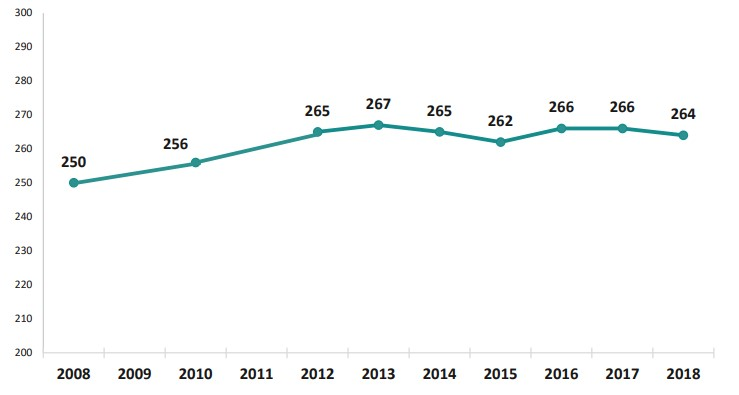
\includegraphics{input/images/trayectoria_sim_mate.jpg}

Fuente: Extraído del informe MINEDUC 2018 elaborado por la Agencia de
Calidad de la Educación

Gráfico 2: Trayectoria del puntaje SIMCE de Lenguaje II medio.

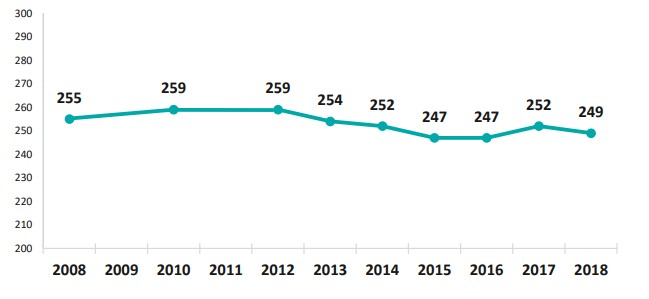
\includegraphics{input/images/trayectoria_sim_leng.jpg}

Fuente: Extraído del informe MINEDUC 2018 elaborado por la Agencia de
Calidad de la Educación

A su vez, la distribución del rendimiento académico se encuentra
fuertemente estratificada en términos sociales. En ese sentido, si
evaluamos los resultados a nivel histórico de la prueba SIMCE de
matemáticas según nivel socioeconómico podremos advertir que hay
diferencias muy pronunciadas entre cada quintil de ingreso. Mientras los
alumnos del quintil más rico promedian 330 puntos, aquellos del quintil
más pobre tan sólo alcanzan, en promedio, 228 puntos. Esta tendencia ha
seguido una trayectoria relativamente estable, pues la brecha que se
genera entre cada grupo es parecida tanto para el año 2008 como 2018
(con sólo 13 puntos de diferencia), así como también en los períodos
comprendidos entre estos años.

Gráfico 3: Puntaje SIMCE Matemática II medio por quintil de ingreso

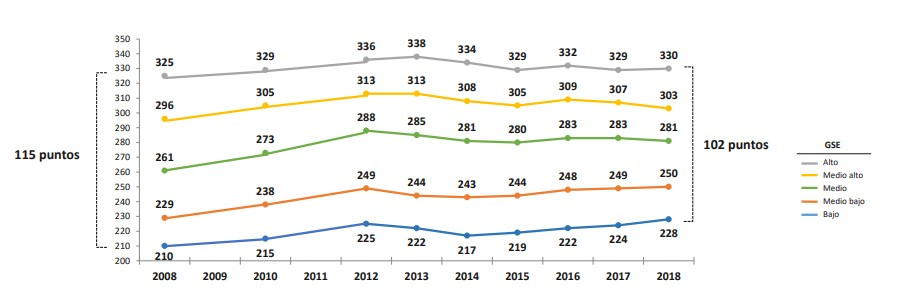
\includegraphics{input/images/puntaje_mate_nse.jpg}

Fuente: Extraído del informe MINEDUC 2018 elaborado por la Agencia de
Calidad de la Educación

En la misma línea, el comportamiento que tiene el rendimiento académico
no es homogéneo si entramos a examinar el género de los estudiantes.
Para el caso de la prueba de lenguaje, las diferencias de puntaje que
hay entre hombres y mujeres alcanzan una proporción alta y cambiante en
el curso de los años. Así, la brecha de género en el aprendizaje de
lenguaje se ha ido acentuando con el paso del tiempo, habiendo 15 puntos
de diferencia entre hombres y mujeres en la última rendición del SIMCE,
en favor de estas últimas. Es interesante mencionar que la brecha de
género constatada en matemática depende de manera importante del
instrumento de medición que se esté utilizando. En ese sentido, a partir
de la prueba PISA y SIMCE es posible observar que la brecha es casi
inexistente (para el caso de PISA la brecha ha ido disminuyendo
sistemáticamente como pueden ver en el gráfico), no obstante, en la
prueba TIMSS, las diferencias de género pueden advertirse con claridad.

Gráfico 4: Brechas de género en prueba SIMCE de Lenguaje II medio

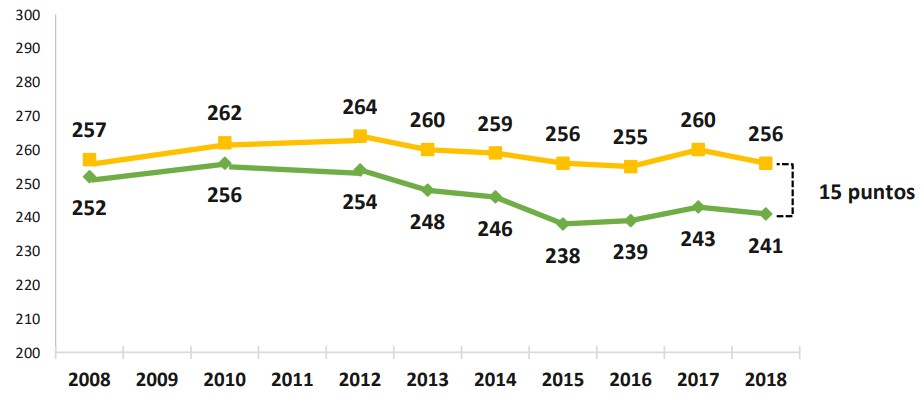
\includegraphics{input/images/brecha_gen_leng.jpg}

Fuente: Extraído del informe MINEDUC 2018 elaborado por la Agencia de
Calidad de la Educación

Gráfico 5: Serie histórica de las brechas de género en prueba PISA de
Matemática

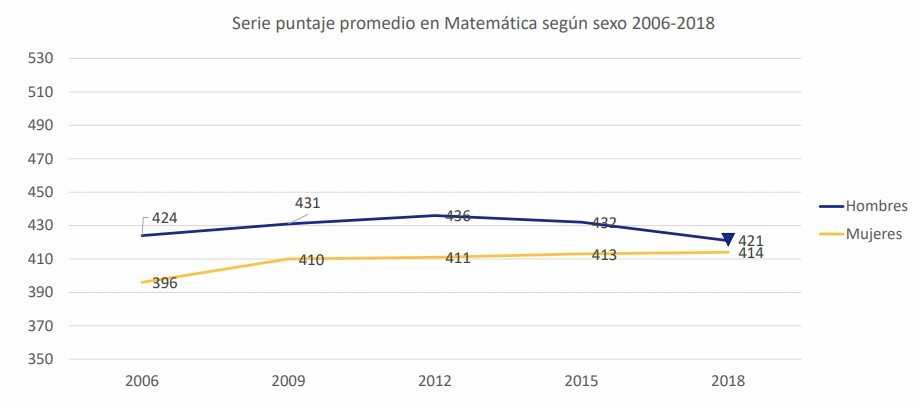
\includegraphics{input/images/brecha_gen_mate_pisa.jpg}

Fuente: Extraído de Informe Agencia de la Calidad de la Educación Pisa
2018

Gráfico 6: Serie histórica de las brechas de género en prueba TIMSS de
Matemática

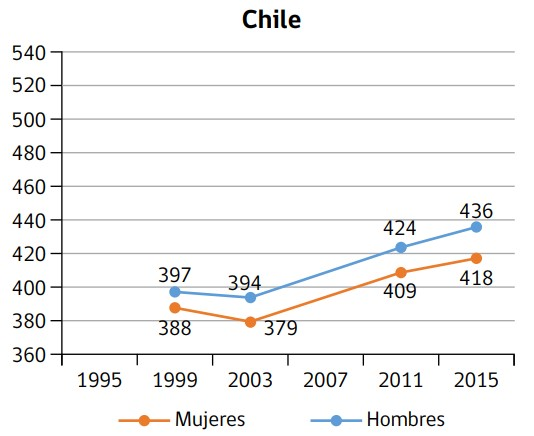
\includegraphics{input/images/brecha_gen_mate_timss.jpg}

Fuente: Extraído de informe nacional de Agencia de la Calidad de la
Educación TIMSS 2015

\hypertarget{acerca-de-la-calidad-educativa-en-el-contexto-de-un-sistema-educativo-desigual}{%
\subsection{Acerca de la calidad educativa en el contexto de un sistema
educativo
desigual}\label{acerca-de-la-calidad-educativa-en-el-contexto-de-un-sistema-educativo-desigual}}

El rendimiento académico en pruebas estandarizadas es una de las muchas
dimensiones que componen una educación de calidad. Teniendo eso a la
vista, el concepto de calidad educativa ha sido objeto de numerosos
debates tanto en la literatura como en organismos asociados a la
supervisión, administración, y regulación de la educación en Chile.

Asociado al modelo de mercado del sistema educacional chileno está la
conceptualización de calidad que hacen algunos economistas inspirados en
la tradición neoclásica. Si bien no enuncian explícitamente una
definición de calidad educativa, es posible identificar una perspectiva
de calidad vinculada a algunos elementos centrales que configuran las
teorizaciones de dichos autores.

En ese sentido, Becker (\protect\hyperlink{ref-becker_human_1993}{1993})
sostiene una mirada acerca de la educación estrechamente vinculada al
concepto de capital humano. De esta forma, el proceso educativo no sería
más que un mecanismo a través del cual se puede aumentar la
productividad de los trabajadores con el propósito de impactar
positivamente en los indicadores económicos de los países. Es decir, una
buena educación sería aquella que produjera individuos más productivos
para el sistema económico imperante, omitiendo cualquier otra dimensión
humana del proceso educativo.

De este modo, se concibe la educación como ``un proceso de aumento de la
productividad del individuo y despojándolo de fundamentos en la sociedad
que habían sido parte del debate educacional del siglo XX y en especial
de aquellos que dicen relación con procesos colectivos y/o
supraindividuales (integración social, valores cívicos, etc.). Así, todo
proceso educativo, afirma Becker, para ser válido y deseado por la
sociedad, debe generar un aumento de capacidades del individuo en el
sistema productivo, particularmente, en el mercado laboral, y su
agregación y articulación con otros individuos escolarizados llevará a
la riqueza de las naciones'' (Alejandro Carrasco,
\protect\hyperlink{ref-alejandrocarrasco_mercado_2016}{2016}, p. 30).

Esta conceptualización va de la mano con el cambio paradigmático
implicado en la gran reforma de municipalización de 1980, la cual
materializa una visión economicista sobre la educación, fundamentada en
las escuelas Austriaca y de Chicago, derivando en una completa
subordinación de la discusión educativa a la tecnocracia neoliberal
compuesta por economistas formados al alero de dichas escuelas
(Alejandro Carrasco,
\protect\hyperlink{ref-alejandrocarrasco_mercado_2016}{2016}).

Esta noción de calidad educativa experimenta un importante vuelco con la
irrupción de las movilizaciones sociales del año 2006 y 2011. Se logra
impugnar la perspectiva hegemónica que subordinaba los procesos y la
calidad educativa a la orientación mercantil que había asumido la
educación chilena. En su lugar, se promueve con fuerza la idea de una
educación comprendida desde su potencial integrativo a nivel social, y
como una dimensión fundamental de la vida humana que debe ser
garantizada por el Estado de Chile (Mayol,
\protect\hyperlink{ref-mayol_derrumbe_2015}{2015}).

En la misma dirección, se plantea que la educación debería ser un
derecho social consagrado para todos los chilenos sin distinción alguna,
cuyo fin sea la promoción activa de la integración social, mediante el
reconocimiento al otro diverso (en sus múltiples ``formas'') como
legítimo, así como también una herramienta igualadora en lo que respecta
a su distribución y provisión (Alejandro Carrasco,
\protect\hyperlink{ref-alejandrocarrasco_mercado_2016}{2016}).

De esta forma, recobra importancia el ideal comunitario que
caracterizaba a la educación del siglo XX. Pues el proceso educativo se
concibe como un proceso de adquisición de ciudadanía, procurando
incentivar la noción de que los individuos forman parte de una misma
comunidad política y, por ende, que deben reconocerse como tal. Esta
visión contrasta totalmente con aquella mercantil que sólo releva el
retorno económico que puede tener la educación (Atria,
\protect\hyperlink{ref-atria_mala_2012}{2012}).

Uno de los principales organismos que ha participado en el debate acerca
del concepto de calidad de la educación es la Agencia de Calidad de la
Educación. Este es un organismo que fue creado el año 2011 con el
propósito de orientar y supervisar el sistema educacional chileno en lo
relativo a la equidad y calidad de la educación de nuestro país.

Recogiendo los amplios debates de la literatura y las heterogéneas
visiones brindadas por los diferentes actores sociales del mundo
educacional, la agencia ha velado por una complejización del constructo
de calidad de la educación. Alineado con ese propósito, la agencia
señala que: ``Se entiende por una educación de calidad un proceso
formativo integral que pone en el centro al ser humano en su totalidad,
promoviendo un desarrollo consistente e integrado del conjunto de
dimensiones, incluyendo la espiritual, la ético-moral, la cognitiva o
intelectual, la afectiva, la artística y la de desarrollo físico, entre
otras, y que se orienta a proveer oportunidades de desarrollo e
integración social al conjunto de los niños y niñas, jóvenes y adultos
de manera equitativa e inclusiva, previniendo la discriminación y la
segregación de cualquier tipo, garantizando que todas y todos puedan ser
ciudadanos autónomos, responsables, proactivos y críticos'' (Plan de
Aseguramiento de la Calidad Escolar 2016-2019, pp.~16).

Con ese insumo teórico, las políticas públicas disponen de un referente
con el cual pueden orientar la evaluación y fiscalización que hacen del
sistema educativo. Cabe destacar que la calidad educativa resulta ser un
constructo que trasciende los buenos rendimientos en pruebas
estandarizadas en las materias tradicionales. Se trata, entonces, de
poner el centro en formar personas integrales que sepan convivir
armoniosamente en una sociedad diversa (Agencia Calidad de la Educación,
2017). Si bien en la presente investigación nos centraremos en la
calidad del proceso educativo asociado a las habilidades cognitivas
(medidas a partir de la prueba SIMCE), no perdemos de vista que es sólo
una de las muchas dimensiones que configuran el aprendizaje de los
alumnos.

Asimismo, es crucial relevar la trascendencia que tiene la inclusión
social en una educación de calidad. De este modo, la preocupación no
debe residir meramente en formar individuos con aptitudes afectivas,
académicas, y cognitivas, sino que también en promover activamente el
respeto hacia el otro y el trato igualitario a los individuos
independiente de su origen social, cultural, étnico, y de género. De
este modo, las escuelas deben centrar su quehacer en hacer de ellas
espacios más inclusivos socialmente, combatiendo así la segregación que
impera en nuestro sistema educacional.

\hypertarget{segregaciuxf3n-social-del-sistema-educacional-chileno}{%
\section{Segregación social del sistema educacional
chileno}\label{segregaciuxf3n-social-del-sistema-educacional-chileno}}

\hypertarget{una-caracterizaciuxf3n-cuantitativa-de-la-segregaciuxf3n-social}{%
\subsection{Una caracterización cuantitativa de la segregación
social}\label{una-caracterizaciuxf3n-cuantitativa-de-la-segregaciuxf3n-social}}

El fenómeno de la segregación social se vincula estrechamente al proceso
educativo que vivencian los estudiantes. Un sistema educacional más
inclusivo, es decir, menos segregado, es socialmente beneficioso para el
conjunto de la sociedad, así como también para los individuos. Cuando
los sujetos comparten en la sala de clases con individuos de origen
social diverso tiene, entre sus consecuencias positivas, desarrollar una
mayor tolerancia hacia sujetos de diversa procedencia social, favorece
la eliminación de estereotipos y estigmas, es un estímulo importante a
la cohesión social de los países, entre otros beneficios (Valenzuela et
al., \protect\hyperlink{ref-valenzuela_evolucion_2008}{2008}).

Además de tener efectos positivos concretos en muchos indicadores de
calidad, una buena educación para todos los individuos independiente de
su origen social es deseable puesto que nos acerca al ideario normativo
de la igualdad de oportunidades (van de Werfhorst,
\protect\hyperlink{ref-vandewerfhorst_changing_2014}{2014}), fuertemente
asentado en las valoraciones morales que hacen los sujetos de las
sociedades occidentales.

Conceptualmente, entenderemos la segregación social como ``la desigual
distribución que poseen los diversos grupos sociales ya sea entre
unidades de organización diferentes, entre zonas geográficas o en una
combinación de ambos, tal que dichas diferencias de distribución afectan
las probabilidades de interacción entre miembros de los diferentes
grupos sociales'' (James \& Taeuber,
\protect\hyperlink{ref-james_measures_1985}{1985}, p. 45).

En consecuencia, la segregación social de un sistema educacional
determinado repercute directamente en el grado de
homogeneidad/heterogeneidad de la composición social de los
establecimientos escolares.

Como consecuencia de la privatización del sistema educacional chileno,
se producen altos niveles de segregación socioeconómica. Siguiendo los
datos obtenidos a partir de la prueba PISA, Chile presenta un nivel de
segregación escolar muy elevado comparado con los 57 países que
participan de la OCDE (González,
\protect\hyperlink{ref-gonzalez_segregacion_2017}{2017}). Concretamente,
nuestro país y Tailandia son los dos países con mayor segregación
socioeconómica del sistema educativo, tomando como referencia al 30\%
más pobre y al 30\% más rico, alcanzando valores sobre 0,5 en el índice
de Duncan (que procederemos a explicar a continuación), cuando la
mayoría de los países se ubican en torno a 0,3-0,4.

En esa línea, se ha estimado que, según el índice de Duncan (medición
utilizada para cuantificar el nivel de interacción entre grupos
sociales, obedeciendo a la definición conceptual recién señalada),
tendríamos una segregación aproximada, para el conjunto del sistema
educacional de 0,5, exhibiendo una de las cifras más altas en
perspectiva comparada como muestra el gráfico 7 (Murillo et al.,
\protect\hyperlink{ref-murillo_evolucion_2018}{2018}). Ahora bien, si
efectuamos el análisis de forma parcelada, según el nivel de ingreso de
cada porción de la sociedad, encontramos que todas las categorías
muestran un grado de segregación significativa, no obstante, quienes se
concentran en la parte alta de la distribución del ingreso son los que
están más segregados (alrededor de 0,6 en el índice mencionado, donde
valores más alto indican un mayor nivel de segregación), esto es, tienen
muchas menos posibilidades de relacionarse con individuos que pertenecen
a grupos sociales que difieren de ellos.

Gráfico 7: Evolución de la segregación socioeconómica en el sistema
educacional por nivel de ingreso

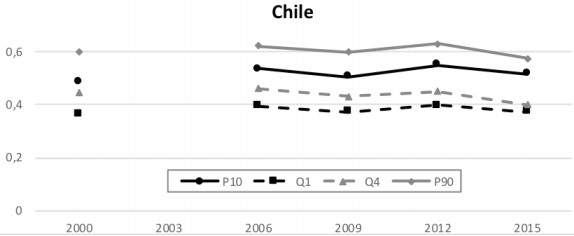
\includegraphics{input/images/evolucion_segregacion_quintiles.jpg}

Fuente: Extraído de Murillo et. al (2018): ``Evolución de la segregación
socioeconómica de las escuelas de América Latina''

Con un propósito similar Bellei
(\protect\hyperlink{ref-bellei_estudio_2013}{2013}) halla que, en
perspectiva comparada, nuestro país es el más segregado tanto social
como académicamente cuando tomamos como punto de comparación los países
que pertenecen a la Organización para la Cooperación y el Desarrollo
Económico (En adelante OCDE). Utilizando una metodología diferente de la
que evalúa la segregación según el ya mencionado índice de Duncan, busca
medir el nivel de homogeneidad/heterogeneidad a partir del nivel
socioeconómico y el capital cultural de los estudiantes de un mismo
establecimiento educacional (estadísticamente corresponde a la varianza
intra-escuela), nuestro país resulta tener el peor nivel de inclusión
social. Por el contrario, Finlandia es el país más integrado socialmente
con un valor de 90 aproximadamente en el índice estandarizado que tiene
por valor máximo el 100, tal como muestra el gráfico 8. En consecuencia,
Chile es un país donde los diferentes estratos socioeconómicos y
culturales tienen muy poco vínculo entre sí, mientras en Finlandia los
diferentes individuos concurren en similar proporción a los
establecimientos constituyéndose en espacios sociales heterogéneos que
permiten el diálogo y la interacción de todos quienes componen a la
sociedad (Bellei, \protect\hyperlink{ref-bellei_estudio_2013}{2013}).

Gráfico 8: Índice de inclusión social y académica para países
perteneciente a la OCDE

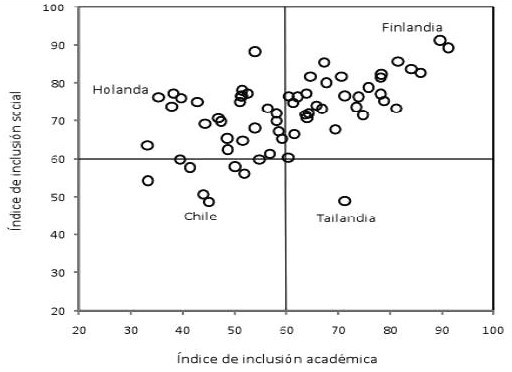
\includegraphics{input/images/inclusion_social.jpg}

Fuente: Extraído de Bellei (2013): ``El estudio de la segregación
socioeconómica y académica de la educación chilena. Estudios
pedagógicos''

\hypertarget{relaciuxf3n-de-la-segregaciuxf3n-social-con-la-composiciuxf3n-de-los-establecimientos}{%
\subsection{Relación de la segregación social con la composición de los
establecimientos}\label{relaciuxf3n-de-la-segregaciuxf3n-social-con-la-composiciuxf3n-de-los-establecimientos}}

Siguiendo esta caracterización más general, es posible constatar que el
elevado nivel de segregación social del sistema educacional chileno se
expresa concretamente en una alta homogeneidad interna de los
establecimientos y, también, una alta heterogeneidad entre las escuelas.
En ese sentido, Villalobos et al.
(\protect\hyperlink{ref-villalobos_composicion_2020}{2020}) señala que
el sistema escolar chileno tendría cuatro grupos de escuelas, agrupadas
a partir de un conjunto de atributos sociales identificados por el autor
(género, etnia, nacionalidad, necesidades educativas especiales, y nivel
socioeconómico). Un grupo de establecimientos concentraría a la élite
del país, en colegios particular pagados, un segundo grupo que agruparía
a estudiantes vulnerables, un tercer grupo que integraría a las clases
medias del país, y un cuarto grupo de establecimientos que tendría un
elevado grado de heterogeneidad social en términos socioeconómicos y
académicos.

Asimismo, la porción de establecimientos heterogéneos se explicaría,
fundamentalmente, por razones académicas, de género, y de ingresos.
Mientras, la cantidad de colegios heterogéneos en lo que respecta a
atributos como etnia, nacionalidad, y necesidades especiales es muy
baja. En efecto, es poco probable que los estudiantes de diversas
culturas y etnias se encuentren en un mismo establecimiento en la medida
que están homogéneamente distribuidos en el sistema educacional. Por el
contrario, estudiantes de diferentes géneros, rendimiento e ingreso
están más mezclados entre sí, produciendo una mayor mixtura social
(Villalobos et al.,
\protect\hyperlink{ref-villalobos_composicion_2020}{2020}).

Analizando en detalle los establecimientos educacionales chilenos,
podemos observar que un 85,2\% es heterogéneo en términos del sexo de
los estudiantes, un 12,29\% es heterogéneo en términos étnicos, y tan
sólo un 5,1\% lo es en lo que refiere a la nacionalidad de los
estudiantes que componen los establecimientos (Villalobos et al.,
\protect\hyperlink{ref-villalobos_composicion_2020}{2020}). Es
interesante destacar que son las cifras más actualizadas acerca de la
composición escolar de los colegios en Chile.

En consecuencia, el sistema escolar chileno estaría altamente
fragmentado en la medida que los diferentes grupos sociales tienen poca
interacción entre sí (con algunas excepciones), obstaculizando el
desarrollo de una mayor cohesión social y el desarrollo de valores
asociados a la aceptación de la diversidad social (Villalobos et al.,
\protect\hyperlink{ref-villalobos_composicion_2020}{2020}).

Con un propósito similar, se ha evidenciado (Ortiz,
\protect\hyperlink{ref-ortiz_escuelas_2015}{2015}) que el sistema
educacional chileno estaría compuesto, a grandes rasgos, por tres tipos
de establecimientos. Habría establecimientos compuestos mayoritariamente
por estudiantes aventajados (34,4\%), establecimientos mixtos o
inclusivos socialmente (22,8\%), y colegios que concentran
predominantemente estudiantes vulnerables o desaventajados (42,8\%).

El modo a partir del cual se genera la tipología de establecimientos
resulta tener importantes arbitrariedades a ser corregidas. La
metodología usada para determinar lo anterior se basa en comparar el
nivel socioeconómico promedio de los establecimientos, con la media
nacional, realizando una prueba T de dos colas para decidir si cada uno
es superior o inferior a dicha media y, conforme a ello, determinar si
es de estudiantes aventajados (nivel socioeconómico sobre la media),
mixto socialmente (cercano a la media socioeconómica nacional) y
compuesto por estudiantes desaventajados (nivel socioeconómico del
establecimiento bajo la media).

En términos étnicos, (Treviño et al.,
\protect\hyperlink{ref-trevino_educacion_2017}{2017}) muestra de qué
forma se generan los patrones de segregación de la población indígena en
Chile. Según este, la segregación de este grupo en particular se
explicaría por razones geográficas, esto es, a raíz de la forma en que
se asienta la población, donde los sectores indígenas tienden a
concentrarse en zonas rurales. De esta forma, habría una diferencia
importante respecto a otras formas de segregación social que venían
dadas, principalmente, por políticas explícitas de los establecimientos
educacionales. Por lo tanto, se concentran de forma importante en las
zonas rurales, lugares en los cuales encontraríamos una mayor
homogeneidad étnica de los establecimientos, mientras en zonas urbanas
dicha homogeneidad interna sería menos acentuada.

\hypertarget{factores-asociados-a-la-segregaciuxf3n-social}{%
\subsection{Factores asociados a la segregación
social}\label{factores-asociados-a-la-segregaciuxf3n-social}}

Respecto a las causas que explican esta elevada magnitud de segregación
la evidencia ha demostrado que uno de los principales factores que
influiría sería la asimetría de información existente entre los
apoderados que eligen las escuelas, mediado por el capital económico y
cultural que disponen (Elacqua,
\protect\hyperlink{ref-elacqua_impact_2012}{2012}). En efecto, las
familias de bajos ingresos elegirían los colegios a partir de criterios
no educacionales, a saber, según cercanía del hogar fundamentalmente,
mientras las familias con mayor capital económico enfocarían su decisión
en la calidad académica de las escuelas (Valenzuela et al.,
\protect\hyperlink{ref-valenzuela_socioeconomic_2014}{2014}). Desde una
perspectiva cualitativa (Hernández \& Raczynski,
\protect\hyperlink{ref-hernandez_eleccion_2015}{2015}), muestran de qué
modo la clase media y baja del país producen dinámicas de exclusión
social. Los sectores medios fundamentan su elección de escuela según la
búsqueda de distinción social, mientras los individuos de familias más
pobres se auto excluyen, reforzando la segregación socioeconómica de la
matrícula. En virtud de lo anterior, se generarían escuelas con altos
niveles de segregación, de manera que las familias pobres quedan
relegadas a escuelas de mala calidad y las familias de altos ingresos a
las mejores escuelas del país.

La segregación residencial existente en las grandes ciudades del país
explicaría una parte importante de la magnitud de la segregación
socioeconómica del sistema educacional (Arteaga et al.,
\protect\hyperlink{ref-arteaga_school_2014}{2014}; Flores,
\protect\hyperlink{ref-flores_consecuencias_2006}{2006}). En efecto, las
estimaciones cifran en alrededor de un 8-13\% de varianza de la
segregación socioeconómica explicada por la segregación residencial,
particularmente para el caso de Santiago.

Si bien la estructuración urbana de las ciudades se relaciona con la
segregación, ciertos autores (Bonal \& Bellei,
\protect\hyperlink{ref-bonal_understanding_2019b}{2019}), mediante
entrevistas a apoderados de diversos estratos socioeconómicos, han
consignado que los mecanismos de mayor impacto estarían mediados por las
dinámicas de mercado del sistema educacional. De este modo, la demanda
de los apoderados por educación para sus hijos tendría orientaciones
fuertemente influenciadas por la composición social de los
establecimientos, buscando espacios con alta homogeneidad interna. En
consecuencia, la clase alta busca establecimientos de composición
sociocultural elitaria, los sectores medios evitan la educación pública
y gratuita para no ``mezclarse'' con familias de bajos ingresos y, estos
últimos, aun cuando una parte importante comparte ese criterio, muchos
de ellos decidirán el colegio de sus hijos según cercanía geográfica.

A su vez, la fisionomía del sistema educativo, edificado a partir de
mecanismos de selectividad, financiamiento compartido, y escuelas
subvencionadas por el Estado respondería a dinámicas de mercado. De esta
manera, se incentivaría a los colegios a elegir y seleccionar
estudiantes de élite y, en el caso de los colegios con fines de lucro,
segmentar también al interior de los colegios de forma tal que los
mejores estudiantes estén conformes (Bellei,
\protect\hyperlink{ref-bellei_expansion_2007}{2007}; Contreras et al.,
\protect\hyperlink{ref-contreras_when_2010}{2010}; Elacqua,
\protect\hyperlink{ref-elacqua_impact_2012}{2012}; Garcia-Huidobro,
\protect\hyperlink{ref-garcia-huidobro_desigualdad_2007}{2007};
Valenzuela et al.,
\protect\hyperlink{ref-valenzuela_evolucion_2008}{2008}).

En la misma dirección, se ha aducido que el factor más relevante que
incide en que un colegio agrupe o no a sus estudiantes tiene relación
con el nivel de heterogeneidad socioeconómica del establecimiento más
que la diversidad académica existente (Treviño et al.,
\protect\hyperlink{ref-trevino_segregacion_2014}{2014}). En coherencia
con lo anterior, aquellos colegios más heterogéneos socialmente realizan
con mayor frecuencia prácticas de agrupamiento que los que tienen una
composición social más homogénea.

Por otra parte, Bellei
(\protect\hyperlink{ref-bellei_estudio_2013}{2013}) ha señalado que la
segregación socioeconómica de las escuelas chilenas se vincularía
positivamente a cuatro factores. Primero, la elevada segregación
residencial que exhibe el país. Segundo, la magnitud de la presencia de
la educación privada no subvencionada en la comuna. Tercero, la
relevancia de los establecimientos particulares subvencionados. Por
último, la relevancia del financiamiento compartido en la comuna.

En síntesis, el sistema escolar chileno está dividido en segmentos
sociales nítidos, como consecuencia de una serie de políticas
educacionales que subyacen al sistema mismo. La combinación de procesos
de admisión selectivos, la elección de los padres, el copago, y la
segregación residencial serían elementos explicativos de la segregación
escolar. En virtud de estos mecanismos, los colegios públicos tenderían
a concentrar a la población socialmente más desaventajada, mientras la
clase media-baja y clase media asistiría a escuelas particulares
subvencionadas (Garcia-Huidobro,
\protect\hyperlink{ref-garcia-huidobro_desigualdad_2007}{2007}).

\hypertarget{efectos-de-la-composiciuxf3n-escolar-en-el-rendimiento-acaduxe9mico}{%
\section{Efecto(s) de la composición escolar en el rendimiento
académico}\label{efectos-de-la-composiciuxf3n-escolar-en-el-rendimiento-acaduxe9mico}}

Habría dos mecanismos centrales mediante los cuales operaría la
segregación social para producir efectos en los logros educacionales
(Bellei, \protect\hyperlink{ref-bellei_estudio_2013}{2013}): por un
lado, a partir de la noción de capital social y, por otro lado, la
teoría del efecto de los compañeros, objeto de interés en la presente
investigación. De este modo, las inequidades en los resultados
educacionales podrían estar asociadas a las consecuencias derivadas de
la composición de los establecimientos, lugar en el cual los integrantes
podrían tener un impacto beneficioso o negativo en los compañeros con
los que comparten el aula escolar.

El modo en que operaría el impacto positivo de una mayor diversidad
étnica, social, económica y de género en el rendimiento académico serían
los siguientes (Dronkers \& van der Velden,
\protect\hyperlink{ref-dronkers_positive_2013a}{2013}): (1) en escuelas
más diversas aquellos estudiantes de un origen privilegiado tenderían a
colaborar con aquellos que tienen mayores problemáticas o bien siendo
una especie de ejemplo para estos últimos; (2) los estudiantes tendrían
mayores posibilidades de enfrentarse a un curriculum desafiante y que
promueva activamente habilidades de todo tipo, pues los profesores
suelen transmitir dichas enseñanzas en contextos en los cuales están los
mejores estudiantes o de origen privilegiado; (3) los estudiantes más
capaces aprenderían más debido al proceso de enseñanza que ellos
practican con los compañeros que requieren que les expliquen las
diferentes materias.

No obstante, también es posible que la diversidad del aula tenga efectos
inhibitorios de un buen rendimiento académico, siendo preferible una
mayor homogeneidad interna. Tres mecanismos se han descrito respecto a
este (Dronkers \& van der Velden,
\protect\hyperlink{ref-dronkers_positive_2013a}{2013}): (1) un cuerpo
estudiantil más homogéneo incrementa las posibilidades de
especialización de los profesores gracias a esa homogeneidad,
propendiendo a una mayor efectividad de la escuela; (2) En aulas más
homogéneas menos tiempo requiere ser gastado en generar puentes entre
los estudiantes de diverso origen cultural y social, permitiendo
destinar ese tiempo a mejorar la enseñanza y el aprendizaje de los
estudiantes; (3) La confianza entre profesores, apoderados, y
estudiantes, en contextos de un cuerpo estudiantil más homogéneo, es
considerablemente mayor propiciando un mayor involucramiento de cada
actor y, por ende, aumentando la efectividad de las escuelas en términos
del aprendizaje resultante de los alumnos.

\hypertarget{efecto-de-composiciuxf3n-socioeconuxf3mica}{%
\subsection{Efecto de composición
socioeconómica}\label{efecto-de-composiciuxf3n-socioeconuxf3mica}}

Antes de indagar en la literatura sobre el tema, es necesario distinguir
dos conceptos que con frecuencia aparecen en la literatura acerca de
composición escolar o efecto par de los compañeros. Por un lado, está el
concepto de composición y, por otro, el de heterogeneidad. Mientras el
primero hace referencia a un promedio o proporción de un atributo
determinado (por ejemplo, el nivel socioeconómico promedio de un aula),
el segundo alude a la dispersión de alguna característica social
definida (Dronkers \& van der Velden,
\protect\hyperlink{ref-dronkers_positive_2013a}{2013}).

La primera aproximación empírica al fenómeno de la composición escolar
referida al nivel socioeconómico data de varias décadas (Coleman,
\protect\hyperlink{ref-coleman_equality_1965}{1965}), quien logró
distinguir, por un lado, la importante influencia que tienen ciertas
características individuales (en inglés, el background), principalmente,
el origen socioeconómico de los individuos de, por otro, el efecto que
tiene la agregación de esta (y otras) características individuales en el
contexto de un establecimiento o sala de clases. De ahí el término de
efecto de composición, estrechamente ligado al nivel socioeconómico
promedio de una sala de clases o establecimiento escolar, según ciertas
variables tradicionales (libros en el hogar, ingreso de los padres,
grado educacional alcanzado por progenitores, etc.).

La discusión acerca de la naturaleza del efecto de composición o mixtura
social reviste de interés mundial. Han sido muchos los países en los
cuales se ha indagado el tópico de composición escolar y rendimiento
académico. Por cierto, es un asunto aún no resuelto, pero sí con algunos
consensos mínimos. Thrupp et al.
(\protect\hyperlink{ref-thrupp_school_2002b}{2002}) sostienen que
después de décadas de investigación acerca de los efectos de composición
o mixtura social de las escuelas, el consenso acerca de la naturaleza y
tamaño de estos efectos es notablemente poco, una conclusión también
evidenciada por muchos otros autores (Angrist \& Lang,
\protect\hyperlink{ref-angrist_does_2004}{2004}; Hoxby,
\protect\hyperlink{ref-hoxby_peer_2000}{2000}; Hoxby \& Weingarth,
\protect\hyperlink{ref-hoxby_taking_2005}{2005}).

En Nueva Zelanda, país donde hay un sistema educacional con un nivel de
estratificación y segregación social relativamente bajo, la varianza del
puntaje entre escuelas es bastante baja. Sólo un 5-9\% de la varianza
del rendimiento de los estudiantes está contenida entre las escuelas.
Sobre ella, tanto la composición cultural (es decir, proporción de
individuos de origen maorí, asiático, y de islas pacificas) como la
composición socioeconómica medida a partir del nivel socioeconómico
promedio del establecimiento tenían casi nula capacidad explicativa de
la varianza entre establecimientos en el puntaje en matemática y
ciencias, alcanzando alrededor de un 1-2\% (Nash \& Harker,
\protect\hyperlink{ref-nash_progress_1997}{1997}). Los autores ponen en
duda la hipótesis de la capacidad explicativa que tendrían variables
composicionales económicas y culturales en relación con las puntuaciones
que obtienen los estudiantes en pruebas estandarizadas.

Algo diferente es posible de advertir en la literatura internacional
acerca del sistema educacional belga. Según Opdenakker \& Damme
(\protect\hyperlink{ref-opdenakker_relationship_2001}{2001}), la
influencia de la composición socioeconómica difiere sustancialmente en
función del estrato en específico que se esté examinando. En particular,
dentro de cada grupo socioeconómico, los estudiantes de mayor habilidad
son más sensibles al cambio de composición socioeconómica del aula que
aquellos de baja habilidad, pues el efecto positivo que tendría un aula
de alto nivel socioeconómico promedio para estudiantes de alta
habilidad, pero de bajo nivel socioeconómico (individual) sería muy
grande, generando, de este modo, un impacto diferenciado de la
composición mediado por la habilidad y el nivel socioeconómico de los
individuos.

En el Reino Unido, uno de los estudios más conocidos en materia de
composición escolar, advierte que, aun cuando encuentran un impacto
sustantivo del nivel socioeconómico promedio del establecimiento en el
rendimiento individual, bien podría ser que ciertos factores no
observables estén incidiendo y explicando esa porción de varianza. El
autoconcepto que tienen los estudiantes de sí mismos, el capital social,
la motivación, el involucramiento de los padres en el proceso educativo
del colegio, todos ellos, elementos que influyen en el proceso de
aprendizaje pero que no correlacionan altamente con el nivel
socioeconómico, razón por la cual podría estar confundiéndose con el
efecto de composición socioeconómica (Nash,
\protect\hyperlink{ref-nash_school_2003}{2003}).

En este mismo país, otro estudio sobre el efecto de composición del
nivel socioeconómico en el rendimiento académico encontró un vínculo
fuerte entre ambos. La varianza de los puntajes entre escuelas se
encontraba explicado en un 25\% por la configuración de clase de los
establecimientos escolares. No obstante, al momento de incorporar
variables asociadas al rendimiento previo y a las habilidades de los
estudiantes, el efecto de composición socioeconómica se cancelaba casi
completamente. De este modo, resulta trascendental integrar para
cualquier análisis acerca del efecto de los compañeros variables que
capturen las habilidades de quienes componen el aula de clases (Gray et
al., \protect\hyperlink{ref-gray_estimating_1990}{1990}).

En la literatura sobre este país, también se ha indicado que los
factores individuales tienen mucho mayor peso explicativo que aquellos
composicionales a nivel escuela. La única materia que se ve afectada por
la composición socioeconómica y étnica es el aprendizaje del lenguaje,
lo cual probablemente, según los autores, estaría ligado a las escuelas
donde hay una alta concentración de migrantes con bajo nivel
socioeconómico. Además, según los resultados observados pareciera ser
que en el nivel más bajo y más alto de la pirámide socioeconómica se
darían, principalmente, los efectos de composición. De este modo, en las
capas medias el nivel socioeconómico no sería tan relevante para efectos
de predecir el rendimiento académico (Sammons et al.,
\protect\hyperlink{ref-sammons_forging_1997}{1997}).

Una serie de advertencias metodológicas sugiere el artículo de van Ewijk
\& Sleegers (\protect\hyperlink{ref-vanewijk_effect_2009}{2009}),
quienes sistematizan una fracción considerable de los estudios
realizados sobre el efecto del nivel socioeconómico de los compañeros.
Según ellos, para obtener estimaciones más precisas de la verdadera
magnitud del impacto que tiene el nivel socioeconómico en el rendimiento
académico es necesario tener algunas precauciones: Primero, medir de
manera íntegra el nivel socioeconómico, pues cuando se construye la
variable con pocos indicadores (por ejemplo, sólo considerando la
cantidad de libros en el hogar y el nivel educacional de los padres) hay
una subestimación significativa del efecto de esta variable; Segundo,
controlar en los modelos de regresión por el rendimiento previo de los
alumnos, para no sobreestimar el impacto del nivel socioeconómico; Por
último, incluir una alta cantidad de covariables para prever la
posibilidad de endogeneidad en el modelo.

A nivel nacional, se ha evidenciado que la segregación socioeconómica
tiene efectos negativos para los resultados académicos de los
estudiantes concentrados en escuelas de bajo NSE, y positivas para
aquellos reunidos en escuelas de alto NSE, hecho ampliamente descrito
por la literatura y confirmado también para el caso de chile (Mizala \&
Torche, \protect\hyperlink{ref-mizala_bringing_2012}{2012}; Valenzuela
et al., \protect\hyperlink{ref-valenzuela_evolucion_2008}{2008}).

En cuanto al efecto que tiene la heterogeneidad social o dispersión
según nivel socioeconómico el estudio de Taut \& Escobar
(\protect\hyperlink{ref-taut_efecto_2012}{2012}) documenta que esta
tiene un efecto positivo sobre el rendimiento de los estudiantes.
Incluso, muestran que aquellas escuelas más diversas socialmente logran
mitigar el impacto negativo que tiene los bajos niveles de ingreso en el
rendimiento de los alumnos. Por otra parte, los estudiantes de más alto
nivel socioeconómico se ven perjudicados, levemente, cuando estudian en
establecimientos heterogéneos, no obstante, la pérdida que muestran es
menor a la ganancia obtenida por los alumnos más desfavorecidos.

Gráficamente, es posible advertir las diferencias en puntaje SIMCE de
individuos de un mismo ingreso económico, pero que asisten a escuelas
que difieren en el grado de heterogeneidad social. Hasta alcanzar un
nivel de ingreso muy alto, es evidente el impacto positivo que tiene
pertenecer a un curso heterogéneo en términos del rendimiento en la
prueba SIMCE. De este modo, sólo individuos que perciben ingresos muy
altos se ven perjudicados por estar en un colegio heterogéneo versus uno
homogéneo.

No obstante, es fundamental advertir que la distinción entre un curso
homogéneo y heterogéneo en términos socioeconómicos que realizan los
autores resulta ser poco precisa en la medida que dicotomiza la
heterogeneidad aun cuando sabemos que esta tiene niveles, pues no se
trata, entonces, de que haya cursos ``homogéneos'' y cursos
``heterogéneos'' sino niveles determinados de esta variable. Otro
elemento interesante de relevar es que la relación analizada supone una
linealidad entre ambas variables, asunto acerca del cual no hay
claridad. Bien podría haber rendimientos crecientes o decrecientes de la
heterogeneidad social como mediador. Por ejemplo, podría ocurrir que a
medida que un individuo provenga de una familia de mayores ingresos, el
efecto positivo o mitigador de estar en un aula heterogénea se vaya
haciendo más pequeño. Son elementos que exploramos en esta
investigación.

Gráfico 9: La heterogeneidad social de las escuelas como moderador del
puntaje SIMCE

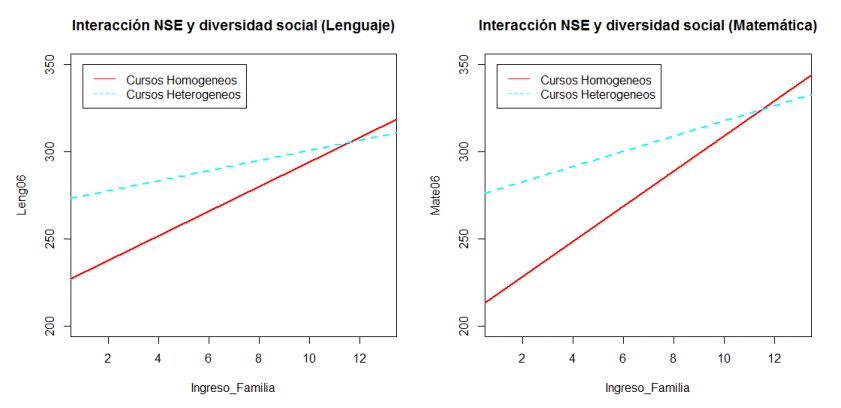
\includegraphics{input/images/heterogeneidad_social_moderador.jpg}

Fuente: Extraído de Taut \& Escobar (2012): ``El efecto de las
características de los pares en el aprendizaje de estudiantes chilenos''

Por último, Ortiz (\protect\hyperlink{ref-ortiz_escuelas_2015}{2015})
mediante un análisis residual de regresión compara los puntajes de
individuos con un mismo background socioeconómico pero que se encuentran
en diferentes colegios según si el colegio es homogéneo o heterogéneo
socialmente. De este modo, el autor observa que las pérdidas en términos
de puntaje debido a la asistencia a uno u otro tipo de establecimiento
tendría una magnitud significativa. Según los hallazgos encontrados, los
estudiantes de los dos primeros quintiles (es decir, el 40\% más pobre)
obtendrían entre 40 y 57 puntos más en la prueba SIMCE cuando se
encuentran en una escuela de alumnos aventajados socialmente en
comparación a lo que obtienen cuando estudian en un colegio de
estudiantes desfavorecidos. Entonces, la inclusión social tendría un
impacto positivo en los estudiantes más pobres sugiriendo la necesidad
de implementar políticas educativas que promuevan la igualdad y equidad
en el sistema escolar.

\hypertarget{efecto-de-composiciuxf3n-de-guxe9nero}{%
\subsection{Efecto de composición de
género}\label{efecto-de-composiciuxf3n-de-guxe9nero}}

Las diferencias de rendimiento según el género son de suma relevancia.
Uno de los principales factores que ha sido aducido como predictor de
las diferencias salariales entre hombres y mujeres es la brecha
existente que tienen en el puntaje de matemática (Koedel \& Tyhurst,
\protect\hyperlink{ref-koedel_math_2012}{2012}).

Uno de los estudios que reviste de mayor robustez en los estudios
educacionales de género concluye que la brecha en matemática se logra
reducir a la mitad cuando, en un mismo establecimiento educacional, las
mujeres se encuentran separadas de los hombres (Paredes,
\protect\hyperlink{ref-paredes_mixed_2018}{2018}). La literatura ha
mencionado que esto podría deberse a que se refuerzan los estereotipos y
prejuicios de género cuando ambos géneros comparten la sala de clases
(Bertrand, \protect\hyperlink{ref-bertrand_new_2011}{2011}).

En la misma línea que Paredes
(\protect\hyperlink{ref-paredes_mixed_2018}{2018}), un estudio efectuado
en el sistema educacional belga tiene hallazgos relativamente similares.
Los investigadores se centran en el efecto que tienen aulas/colegios en
las que hay un sólo género y aulas compartidas en el rendimiento que
tienen hombres y mujeres en matemática y lenguaje (Van de gaer et al.,
\protect\hyperlink{ref-vandegaer_effects_2004}{2004}). Para los hombres,
la composición de género de la clase tiene más impacto que la
composición de género del colegio, mientras que para las mujeres ocurre
al revés. En consecuencia, los hombres incrementan su rendimiento en
lenguaje (y no en matemáticas) en aulas mixtas y a las mujeres, les va
mejor en matemática (pero no en lenguaje) en colegios de un sólo género
que en colegios mixtos.

Dumay \& Dupriez (\protect\hyperlink{ref-dumay_does_2008}{2008}),
también para el caso belga, obtienen resultados relativamente similares.
La mixtura por género no tiene un efecto positivo en el aprendizaje en
matemática para los hombres, pero sí en sus resultados en lenguaje. Al
mismo tiempo, los colegios mixtos perjudican el aprendizaje de
matemática de las mujeres quienes obtienen peores resultados en este
tipo de establecimientos.

Un estudio para Estados Unidos realizado en la zona de Texas encuentra
que una mayor heterogeneidad de género en términos de mayor proporción
de mujeres en el aula produce un efecto positivo en el rendimiento de
matemática de los hombres, sin afectar de modo significativo el
resultado obtenido por las mujeres de la misma sala de clases (Hoxby,
\protect\hyperlink{ref-hoxby_peer_2000}{2000}).

Evidencia algo contradictoria encuentran otros autores que han indagado
en tópicos de género. Según Villalobos et al.
(\protect\hyperlink{ref-villalobos_composicion_2016}{2016}) la
composición de género no desempeña un papel primordial en las dos
variables recién mencionadas. De esta forma ``la educación exclusiva
para un solo género en Chile no genera mejores resultados académicos ni
tiene efectos claros en el ambiente social escolar, dando así cuenta de
la necesidad de incorporar la variable de género como un componente
fundamental de la inclusión educativa'' (Villalobos et al.,
\protect\hyperlink{ref-villalobos_composicion_2016}{2016}, p. 10).

Similar a lo hallado por Villalobos, una serie de estudios
internacionales han encontrado resultados afines. A partir de Bone
(\protect\hyperlink{ref-bone_girls_1983}{1983}), en su estudio acerca de
la diferencia en términos de rendimiento académico de los
establecimientos educacionales de los colegios de un solo género para
alumnos británicos, identifica que las diferencias son mínimas una vez
que se controla por ciertas variables, especialmente, aquellas asociadas
a los procesos de admisión.

En Irlanda, se respalda la hipótesis anterior, en virtud de los
hallazgos obtenidos por Hannan et al.
(\protect\hyperlink{ref-hannan_coeducation_1996}{1996}). No hay
diferencias significativas en el rendimiento académico cuando comparamos
colegios mixtos con colegios no mixtos. Esta discusión reviste de una
importancia trascendental en Irlanda en la medida que alrededor de un
tercio de los establecimientos se componen de alumnos de un solo género.

Con el espíritu de sistematizar los hallazgos vinculados a las
diferencias de rendimientos entre colegios mixtos y no mixtos Smyth
(\protect\hyperlink{ref-smyth_singlesex_2010}{2010}) subraya que, de 39
estudios revisados sobre el tópico, 23 de ellos encontraban un efecto
casi nulo o insignificante de la composición de género mixta, en 15 de
ellos había resultados favorables a una composición de un solo género, y
tan sólo uno del total de los estudios tenía resultados positivos para
establecimientos mixtos.

En el mismo campo de estudio, Taut \& Escobar
(\protect\hyperlink{ref-taut_efecto_2012}{2012}) encuentran que a las
mujeres les va peor comparativamente que a los hombres en matemática y a
estos últimos mejor en lenguaje cuando se encuentran en colegios mixtos.
A su vez, otro resultado interesante a destacar es que una mayor
proporción de mujeres en la sala de clases se asocia con un mayor
rendimiento en matemática de los hombres, no obstante, siguen exhibiendo
peores métricas que los hombres (en matemática).

Consistente con los resultados encontrados por Taut y Escobar, Radovic
Sendra (\protect\hyperlink{ref-radovicsendra_diferencias_2017}{2017})
prueba que las diferencias de rendimiento en matemática entre niñas y
niños son persistentes en el tiempo según la prueba SIMCE, pues tanto
los alumnos de cuarto como de octavo básico muestran diferencias
significativas. No obstante, el género del o la estudiante sólo logra
explicar un 1\% de la varianza de los resultados. Asimismo, las
diferencias de género sólo alcanzan, como máximo, un 20\% de una
desviación estándar. Por último, un resultado novedoso que exhibe el
estudio es la interacción significativa entre el género y el nivel
socioeconómico de los estudiantes. En ese sentido, las diferencias de
género en matemática van decreciendo a medida que los individuos tienen
un mayor nivel socioeconómico.

\hypertarget{efecto-de-composiciuxf3n-migrante-y-uxe9tnica}{%
\subsection{Efecto de composición migrante y
étnica}\label{efecto-de-composiciuxf3n-migrante-y-uxe9tnica}}

La literatura internacional muestra que los estudiantes que sufren de
mayor segregación étnica y racial tienen bajos rendimientos en tareas de
tipo intelectual, baja motivación y bajos niveles de formación cívica
(McEwan, \protect\hyperlink{ref-mcewan_can_2008}{2008}).

La investigación en composición étnica y migrante proviene,
fundamentalmente, de Europa. La evidencia nos señala que hay un consenso
establecido acerca de los efectos positivos que tiene para las minorías
étnicas el pertenecer a escuelas con mayor mixtura pero evidencia más
contradictoria con respecto al eventual efecto negativo en el desempeño
logrado por las minorías étnicas cuando se encuentran en
establecimientos con bajo nivel de diversidad étnica-cultural
{[}Driessen (\protect\hyperlink{ref-driessen_ethnicity_2001}{2001});
Dronkers \& Levels (\protect\hyperlink{ref-dronkers_school_2007}{2007});
Szulkin \& Jonsson (\protect\hyperlink{ref-szulkin_ethnic_2007}{2007});
van Ewijk \& Sleegers
(\protect\hyperlink{ref-vanewijk_effect_2009}{2009}); Van Houtte \&
Stevens (\protect\hyperlink{ref-vanhoutte_school_2010}{2010}); Agirdag
et al. (\protect\hyperlink{ref-agirdag_why_2012}{2012})).

El caso estadounidense es ilustrativo al respecto. Aun cuando se han
implementado elaboradas políticas de inclusión étnica y migrante en
términos de propender hacia una mayor mixtura social, la evidencia
empírica acumulada para este país ha logrado demostrar que las
diferencias en aprendizaje entre estudiantes migrantes y no migrantes se
logran reducir de forma más pronunciada cuando los migrantes se
encuentran en establecimientos homogéneos, esto es, con sujetos del
mismo origen étnico (es importante aclarar que, en la literatura
internacional, dentro de un mismo grupo étnico se consideran varios
países. Por ejemplo, el grupo étnico o racial ``asiático'' incluye
países como corea del sur y japón) (Merry \& Driessen,
\protect\hyperlink{ref-merry_equality_2012}{2012}).

Uno de los programas de inclusión social más importantes que se han
hecho en EEUU, buscando equilibrar cuantitativamente una composición
cultural mixta, encontró resultados interesantes. El programa,
denominado METCO, realizado en la ciudad de Boston de Estados Unidos,
consistía en transferir estudiantes de colegios con una concentración de
alumnos no blancos mayor a 50\% a establecimientos con una proporción de
estudiantes no blancos menor a 30\%. Los resultados de la investigación
señalan (Angrist \& Lang,
\protect\hyperlink{ref-angrist_does_2004}{2004}), contrario a la mayoría
de la evidencia en la materia, que un aumento de las minorías
étnicas/culturales en la sala de clases no produce una merma en el
rendimiento de la mayoría de los estudiantes. Además, de los efectos
observados, el único que pareciera ser relevante, aunque de baja
magnitud, sería el impacto negativo de la composición racial en la
población negra que ya se encontraba en los establecimientos en los
cuales se produjo la llegada de estudiantes del programa METCO (Esto es,
estudiantes no-blancos que se hallaban en colegios con alta
concentración de pares similares).

En Inglaterra, se llevó a cabo un estudio (Smyth,
\protect\hyperlink{ref-smyth_singlesex_2010}{2010}) en 18 escuelas con
una composición multiétnica cada una, testeando la hipótesis del efecto
que poseía la mixtura cultural. La investigación constata que tanto la
puntuación obtenida en matemática como la obtenida en lenguaje no se ve
afectada por la composición étnica pero sí por el rendimiento previo que
tenían los alumnos y también por la proporción de estudiantes de alto
logro en la sala de clases.

En Suecia se efectuó un estudio que documenta el impacto negativo que
tiene la alta concentración de estudiantes migrantes en las escuelas en
el rendimiento tanto de ellos mismos como de estudiantes nativos. Logran
demostrar que cuando hay una concentración o densidad étnica mayor a
40\% en la sala de clases, es decir, una proporción de estudiantes
migrantes que supere ese límite genera fuertes efectos negativos en las
notas que obtienen los estudiantes del establecimiento. De este modo, se
sugiere que políticas educativas que contrarresten la segregación
generaría impactos positivos tanto en términos de eficiencia como de
reducción de la brecha educacional entre los estudiantes (Szulkin \&
Jonsson, \protect\hyperlink{ref-szulkin_ethnic_2007}{2007}).

Harker \& Tymms (\protect\hyperlink{ref-harker_effects_2004}{2004}), en
su estudio acerca del sistema educacional neozelandés constatan que la
varianza que hay en el puntaje de los individuos entre escuelas se
explica casi exclusivamente por el nivel socioeconómico promedio de los
establecimientos educacionales. El rendimiento previo de los estudiantes
y el grado de concentración étnica es irrelevante en términos
estadísticos para efectos de capturar la varianza de puntaje entre las
escuelas de Nueva Zelandia. Es interesante subrayar que encuentran un
impacto similar para las tres pruebas tradicionales aplicadas, a saber,
lenguaje, matemática, y ciencias.

Con una lógica similar, un estudio acerca del sistema educacional alemán
(Van der Slik et al.,
\protect\hyperlink{ref-vanderslik_ethnic_2006}{2006}) integra en su
medición del efecto composición el nivel socioeconómico promedio del
aula y la proporción de estudiantes de otras etnias. Los resultados
indican que los estudiantes que están en salas de clases con una alta
proporción de estudiantes de otras etnias obtienen peores resultados en
las pruebas de lenguaje que aquellos estudiantes que están en aulas con
baja proporción de estudiantes de diverso origen étnico. Lo interesante
del estudio es que al momento de perfeccionar la medición del estatus
socioeconómico promedio (añadiendo variables como si la madre está
empleada y la variación de los ingresos del padre en el último tiempo),
el impacto de la composición étnica deja de ser significativo.

Indagando con mayor precisión en el efecto de la presencia de
inmigrantes en la sala de clases, Contini
(\protect\hyperlink{ref-contini_immigrant_2013}{2013}) prueba que una
mayor concentración de migrantes tiene un efecto negativo pero
diferenciado en el rendimiento académico de los alumnos. De este modo,
los migrantes se ven más perjudicados que los nativos por la presencia
de migrantes y, entre los nativos, aquellos de nivel socioeconómico más
bajo experimentan una mayor baja en su rendimiento que el resto. Todos
los efectos negativos encontrados tienen una magnitud baja, razón por la
cual las preocupaciones acerca de una eventual merma significativa en
las puntuaciones académicas de los italianos, producto de la oleada de
inmigrantes, carece de fundamentos empíricos.

Tomando como referencia el sistema educacional de 17 países europeos,
Dronkers \& van der Velden
(\protect\hyperlink{ref-dronkers_positive_2013a}{2013}), someten a
contraste empírico la influencia que tiene la diversidad cultural
(incluyendo la etnia y el origen migrante), en el rendimiento académico
de estudiantes nativos como de origen migrante, encontrando resultados
ostensiblemente ambivalentes. Por un lado, aseveran que una mayor
diversidad étnica de la sala de clases produce una merma considerable
del puntaje obtenido en habilidades idiomáticas de estudiantes con
origen migrante. Mientras, para los estudiantes nativos, el efecto
negativo de la diversidad étnica sólo ocurre en aquellos países con
sistemas educacionales altamente estratificados en términos sociales.

Por otro lado, la presencia de ciertos grupos étnicos generaría efectos
positivos en el aprendizaje del conjunto diverso que compone la sala de
clases. Concretamente, la presencia de estudiantes asiáticos (no
islámicos) aumentaría el puntaje obtenido en pruebas de idioma de
individuos nativos, inmigrantes no asiáticos, y también en los mismos
migrantes asiáticos no islámicos. El efecto más fuerte de la presencia
de alumnos asiáticos sería para los mismos alumnos asiáticos, aumentando
en 16 puntos por cada 10\% adicional de estudiantes que provengan de esa
región. Por su parte, para inmigrantes no asiáticos y alumnos nativos el
grado de influencia sería de 7 y 5 puntos respectivamente cada 10\%
adicional de asiáticos no islámicos.

Se vuelve fundamental relevar que para ninguno de los otros grupos
étnico/migrantes analizados en el estudio se observa un patrón de
relación positiva como el que hay a partir de la presencia de migrantes
asiáticos no islámicos. Por el contrario, la presencia de estudiantes
del Oeste de Europa impacta negativamente en los resultados obtenidos en
idiomas por los estudiantes nativos (Dronkers \& van der Velden,
\protect\hyperlink{ref-dronkers_positive_2013a}{2013}). Como sugerencia
de política educativa, teniendo a la vista 17 sistemas educacionales de
los países más influyentes del continente europeo, se encuentra
evidencia contradictoria acerca de las consecuencias derivadas de la
mixtura cultural en el rendimiento académico. Pareciera ser que hay
determinadas circunstancias en las cuales una mayor homogeneidad
cultural puede traer resultados positivos para los estudiantes (ejemplo
de estudiantes asiáticos no islámicos que potencian fuertemente el
rendimiento de estos a medida que aumenta su presencia).

El estudio detallado de la composición cultural de las escuelas en Chile
no ha recibido mayormente la atención de los especialistas. Uno de los
más importantes antecedentes académicos (de carácter cualitativo) donde
se investiga la sala de clases enfatizando en las culturas migrantes
(Riedemann \& Stefoni,
\protect\hyperlink{ref-riedemann_sobre_2015}{2015}; Tijoux,
\protect\hyperlink{ref-tijoux_escuelas_2013}{2013}) concluye que los
estudiantes de origen inmigrante están expuestos constantemente a
fuertes prejuicios y modos de discriminación que propician un ambiente
escolar hostil para ellos. En consecuencia, es posible inferir que, aun
cuando no orientan el estudio desde una perspectiva en la dirección aquí
planteada, proporcionan ciertas luces sobre la conflictiva integración
de las culturas subalternas en la sala de clases, insinuando una
eventual relación negativa de escuelas mixtas culturalmente y las
puntuaciones obtenidas por las minorías culturales.

Asimismo, el nivel de integración de los migrantes difiere según el país
de origen de cada uno de ellos (Castillo et al.,
\protect\hyperlink{ref-castillo_estudiantes_2018}{2018}). Quienes se
encuentran más marginados, en términos de relaciones de amistad, son
aquellos de procedencia haitiana y colombiana, mientras que los
bolivianos y peruanos están más integrados en las salas de clases. Según
los hallazgos, las tensiones producidas al interior de la sala de clases
entre nacionales y migrantes ocurren con mayor frecuencia para el caso
de haitianos y colombianos. De todos modos, los resultados sugieren que,
a nivel genérico, cuando la proporción de migrantes y no migrantes está
más equilibrada o con mayor concentración migrante, los conflictos en la
sala de clases son mayores.

La investigación más reciente en temas de inclusión educativa de la
población migrante, consigna que hay un sesgo sistemático de parte de
los docentes a interactuar menos con alumnos que tengan origen migrante,
en la asignatura de matemáticas (Ortega et al.,
\protect\hyperlink{ref-ortega_centrality_2020}{2020}). También, es
importante destacar a partir de la investigación, que aquellas aulas con
mayor composición migrante no logran generar, de forma consistente, una
mayor interacción alumno-docente para el caso de los migrantes.

En materia étnica, la primera contribución en la materia (McEwan,
\protect\hyperlink{ref-mcewan_indigenous_2004}{2004}) advierte una
diferencia de puntaje que se ubica en torno a 0.3-0.5 desviaciones
estándar entre población mapuche y no mapuche. La investigación tiene
algunas deficiencias importantes, pues determina el origen étnico
considerando si la madre pertenece a la etnia mapuche o no. De esta
forma, sugieren la relevancia de considerar los efectos de composición
étnica para poder dilucidar las diferencias existentes entre
establecimientos públicos y privados.

Undurraga (\protect\hyperlink{ref-undurraga_unraveling_2014}{2014}), en
su tesis doctoral, utiliza una medición distinta para identificar a los
alumnos mapuche. Tomando como proxy la auto identificación étnica de los
padres, constatan que las diferencias entre mapuches y no mapuches en el
SIMCE se encuentran entre las 0,2-0,3 desviaciones estándar, según la
prueba que se considere. Una de las principales variables que explicaría
esta diferencia sería el nivel socioeconómico individual de los
estudiantes, mientras que la composición étnica tendría un efecto
negativo en el rendimiento en matemática y ciencias, que vendría
mediado, según lo señalado por el autor, por las bajas expectativas que
tienen los docentes de sus alumnos cuando hay una alta concentración de
estudiantes indígenas.

Asimismo, Cerda (\protect\hyperlink{ref-cerda_situacion_2009}{2009})
confirma que la población mapuche en la Región de la Araucanía (aquella
que recoge la mayor cantidad de estudiantes mapuches en Chile) tiene la
menor escolaridad promedio y, al mismo tiempo, tiene los puntajes SIMCE
más bajos de la región.

Por último, Canales \& Webb
(\protect\hyperlink{ref-canales_educational_2018}{2018}) visualizan el
efecto negativo que tiene la concentración étnica para los estudiantes
indígenas. Al cargar con muchas inequidades los estudiantes de este
grupo, pues concentran mayores niveles de desmotivación, la calidad de
los profesores suele ser más baja, los recursos tanto económicos,
culturales, como institucionales son deficientes, su aprendizaje se ve
radicalmente afectado. Los mismos autores encuentran que sujetos de
origen indígena en aulas diversas o mixtas socialmente tienen muchos
mejores resultados en comparación a lo que obtienen en escuelas que
acogen a un gran porcentaje de estudiantes indígenas.

\hypertarget{objetivos-de-investigaciuxf3n}{%
\section{Objetivos de
investigación}\label{objetivos-de-investigaciuxf3n}}

\textbf{Objetivo general de investigación:}

Determinar en qué medida el grado de heterogeneidad de la composición
escolar en términos culturales, socioeconómicos y de género, se
relaciona con el rendimiento en matemática y lenguaje de estudiantes
mujeres, indígenas, migrantes, y de bajo nivel socioeconómico de II
medio.

\textbf{Objetivos específicos:}

\begin{enumerate}
\def\labelenumi{(\arabic{enumi})}
\tightlist
\item
  Evaluar la relación que tiene la heterogeneidad socioeconómica de los
  establecimientos escolares con el rendimiento académico de los
  estudiantes de niveles socioeconómicos más bajos.
\item
  Evaluar la relación que tiene la composición de género de los
  establecimientos escolares con el rendimiento de las mujeres en
  matemática y lenguaje.
\item
  Evaluar la relación que tiene la heterogeneidad migrante/étnica de los
  establecimientos escolares con el rendimiento de indígenas y migrantes
  en matemática y lenguaje.
\end{enumerate}

\hypertarget{hipuxf3tesis-de-investigaciuxf3n}{%
\section{Hipótesis de
investigación}\label{hipuxf3tesis-de-investigaciuxf3n}}

\begin{enumerate}
\def\labelenumi{(\arabic{enumi})}
\tightlist
\item
  Los alumnos de niveles socioeconómicos más bajos se ven más
  favorecidos de establecimientos heterogéneos socioeconómicamente que
  aquellos alumnos de niveles socioeconómicos más altos.
\item
  Las mujeres se ven beneficiadas en términos del rendimiento que tienen
  en matemática cuando se encuentran en colegios no mixtos, mientras en
  lenguaje no hay un efecto significativo de una composición de estas
  características.
\item
  Los indígenas y migrantes obtienen mejores resultados cuando se
  encuentran mezclados con individuos de origen étnico y nacionalidad
  diverso que cuando están homogéneamente concentrados.
\end{enumerate}

\hypertarget{metodologuxeda}{%
\section{Metodología}\label{metodologuxeda}}

\hypertarget{datos}{%
\subsection{Datos}\label{datos}}

La investigación utilizará datos cuantitativos provenientes de fuentes
secundarias. Particularmente, se usa información del Sistema Integral de
Mejoramiento de la Calidad Educativa (SIMCE). El SIMCE es una prueba
(que evalúa las habilidades en Matemática, Ciencias Naturales, Ciencias
Sociales, y Lenguaje) que se aplica todos los años, de carácter censal,
a estudiantes de 4to, 8vo, y 2do Medio, junto con una serie de
cuestionarios que recolectan información de los profesores, apoderados,
y los mismos alumnos.

Específicamente, son pruebas de conocimientos curriculares en varios
subsectores en la cual no existe una escala estandarizada, sin embargo,
para aspectos generales se considera una escala de un mínimo de 100 y un
máximo de 400 puntos, con un promedio de 250 y una desviación estándar
de 50 puntos. Además de la prueba de conocimientos curriculares, SIMCE
recoge información de contexto a través de un cuestionario para los
padres de los estudiantes testeados. Este cuestionario tiene como fin
indagar sobre el nivel educacional de los padres, el ingreso del hogar,
el nivel de satisfacción con el establecimiento, nacionalidad (tanto de
padres/madres como alumnos), origen étnico (tanto de padres/madres como
de alumnos), entre otros. Usaremos los datos correspondientes para los
alumnos que rindieron la prueba en 2do Medio el año 2017.

Las dos fuentes de información usadas, esto es, el cuestionario de los
padres y los datos sobre el puntaje de los estudiantes difieren en la
cantidad de observaciones. Mientras esta última cuenta con información
de 245.197 estudiantes que rindieron la prueba SIMCE, el cuestionario de
los padres sólo logra cubrir a 169.824 estudiantes. Como consecuencia de
lo anterior, se trabaja, en principio, con 169.824 observaciones. Luego
de la limpieza de los datos y considerando los datos pérdidos la muestra
con la cual realizamos los analisis es de 147.979 estudiantes
distribuidos en 2901 establecimientos a nivel nacional.

\hypertarget{variables}{%
\subsection{Variables}\label{variables}}

Tabla 1: Variables independientes a nivel escuela

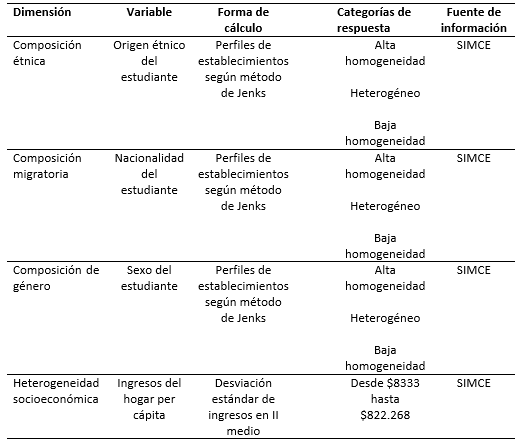
\includegraphics{input/images/VI_ESCUELA.png}

En la tabla adjunta podemos advertir las variables independientes
sustantivas de interés. En cada una de ellas, se especifica la forma de
cálculo, las categorías de respuesta resultante, y la fuente de
información utilizada para extraerlas. Aquí solo enunciaremos cada uno
de estos elementos, pues en la sección metodológica se detallará la
forma de construcción de variables, las respuestas posibles, y todos los
elementos asociados a nuestras variables teóricamente relevantes.

Tabla 2: Variables independientes a nivel individual\\
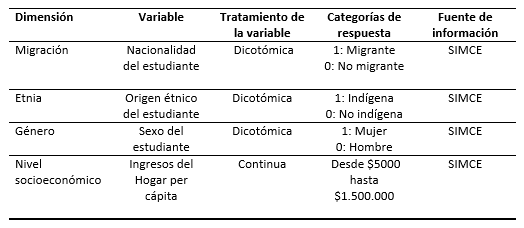
\includegraphics{input/images/VI_INDIVIDUO.png}

Por otra parte, tenemos las variables independientes sustantivas de
orden individual. Al tratarse de datos jerarquizados o de dos niveles,
es fundamental distinguir las variables que corresponden a cada uno de
los niveles. Mientras en la tabla 1 se mostraron las variables asociadas
a los establecimientos escolares, la tabla 2 nos exhibe las variables a
nivel individual. Como podrán notar, estas revisten de mayor
simplicidad, tanto en su forma de cálculo como en las categorías de
respuesta.

Por último, esta investigación tiene como variables dependientes el
puntaje obtenido en la Prueba SIMCE Matemática y el obtenido en la
Prueba SIMCE Lenguaje 2017

\hypertarget{anuxe1lisis}{%
\subsection{Análisis}\label{anuxe1lisis}}

Se estimarán modelos lineales jerárquicos, más conocidos como modelos
multinivel para examinar la relación entre las variables a nivel
establecimiento escolar (nivel 2) y variables a nivel estudiante (nivel
1), con el puntaje en prueba SIMCE de Matemática y Lenguaje que muestran
los estudiantes. La ventaja de este método de estimación radica en la
posibilidad de descomponer la varianza de los puntajes de los alumnos
entre escuelas, por un lado, y dentro de las escuelas por otro. Lo
anterior es posible debido a que los métodos multinivel consideran la
estructura anidada de los datos (en este caso alumnos que se encuentran
anidados en establecimientos escolares). En ese mismo sentido, permite
modelar independientemente la variabilidad en los distintos niveles de
agregación y la interacción entre estos niveles.

\hypertarget{descripciuxf3n-de-variables}{%
\subsection{Descripción de
variables}\label{descripciuxf3n-de-variables}}

\hypertarget{variables-nivel-estudiante}{%
\subsubsection{Variables nivel
estudiante}\label{variables-nivel-estudiante}}

\% Table created by stargazer v.5.2.2 by Marek Hlavac, Harvard
University. E-mail: hlavac at fas.harvard.edu \% Date and time: vie.,
dic. 11, 2020 - 23:22:11

\begin{table}[!htbp] \centering 
  \caption{Descriptivos nivel estudiante} 
  \label{} 
\begin{tabular}{@{\extracolsep{5pt}}lccccccc} 
\\[-1.8ex]\hline 
\hline \\[-1.8ex] 
Statistic & \multicolumn{1}{c}{N} & \multicolumn{1}{c}{Mean} & \multicolumn{1}{c}{St. Dev.} & \multicolumn{1}{c}{Min} & \multicolumn{1}{c}{Pctl(25)} & \multicolumn{1}{c}{Pctl(75)} & \multicolumn{1}{c}{Max} \\ 
\hline \\[-1.8ex] 
rbd & 147,979 & 11,308.480 & 8,821.320 & 1 & 4,286 & 16,441 & 40,457 \\ 
puntaje\_leng & 147,979 & 254.803 & 51.122 & 116.780 & 217.890 & 291.380 & 397.290 \\ 
puntaje\_mate & 147,979 & 270.224 & 63.388 & 96.590 & 223.905 & 317.640 & 428.040 \\ 
ingresos & 147,979 & 167,611.400 & 185,102.600 & 5,000 & 62,500 & 180,000 & 1,500,000 \\ 
sexo & 147,979 & 0.511 & 0.500 & 0 & 0 & 1 & 1 \\ 
cultura & 147,979 & 0.211 & 0.408 & 0 & 0 & 0 & 1 \\ 
educacion & 147,979 & 12.230 & 2.605 & 0 & 12 & 14 & 17 \\ 
nacionalidad & 147,979 & 0.045 & 0.207 & 0 & 0 & 0 & 1 \\ 
etnia & 147,979 & 0.174 & 0.379 & 0 & 0 & 0 & 1 \\ 
\hline \\[-1.8ex] 
\end{tabular} 
\end{table}

Si observamos la tabla, contiene todas las variables a nivel estudiante
que son de interés en este estudio. Respecto al sexo de los individuos,
tenemos que hay casi la misma proporción de hombres y mujeres en la
muestra considerada. Los ingresos del hogar, a su vez, utilizados para
medir el nivel socioeconomico de los alumnos se construyó a partir de
dos variables siguiendo el esquema descrito a continuación: Por una
parte, contamos con la variable de ingresos por tramo (siendo el tramo
de menor ingreso equivalente a ``ganar menos de \$100.000'', y el tramo
de mayor ingreso igual a ganar más de \$2.200.000, con otros trece
tramos entre ellos), por otra, con la cantidad de habitantes del hogar.
Se imputó a cada estudiante el valor medio entre el rango inferior y
superior de cada tramo y, para el caso de la categoría más baja y más
alta se imputó la cantidad de \$50.000 y \$3.000.000 respectivamente.
Posteriormente, se dividió el monto en cuestión por la cantidad de
habitantes del hogar del estudiante.

A partir de la distribución de la variable podemos notar nítidamente que
hay una marcada concentración de los datos hacia la izquierda, cuya
asimetría podemos explicar a partir de los bajos ingresos, en promedio,
de la población chilena. Más especificamente, la media nacional de
ingresos del hogar per cápita alcanza el valor de casi 170 mil pesos,
mientras que la mitad de la población gana menos de 110 mil, dando
cuenta de la existencia de ingresos mediano-bajos a nivel país. La
asimetría de la variable es muy elevada, con una fuerte concentración de
los individuos a la izquierda de la distribución.

Por su parte, para medir el origen cultural de los estudiantes
(considerando etnia y nacionalidad), generamos tres variables.
Primeramente, la etnia y nacionalidad por separado de modo que podamos
cuantificar la cantidad de estudiantes indigenas y migrantes que hay en
la matricula secundaria a nivel nacional. Sólo u 4.5\% de la matricula
es de una nacionalidad diferente a la chilena, mientras un 16.6\% tiene
origen índigena.

Para decidir si un estudiante era índigena o migrante se tomó como
referencia al padre, la madre, y al estudiante mismo. Si en alguna de
las tres preguntas se indicaba que era indigena o migrante se le
imputaba origen etnico/migrante. Luego, para construir la variable
composición cultural se consideró ambas variables siguiendo el mismo
criterio: si los padres indicaban en al menos una de las seis preguntas
en cuestión ser migrante o índigena se le imputaba un origen cultural
diverso. Por esta razón, los estudiantes diversos culturalmente no se
componen por la suma ordinaria de ambas variables (pues hay algunos que
cumplen ambas condiciones), alcanzando un 20.4\% de la matricula
nacional.

Ahora bien, si penetramos en las variables dependientes del estudio,
tenemos un comportamiento de las variables algo diferente a las
anteriores. En primer lugar, los resultados en matematica tienen una
mayor variabilidad que los puntajes en la prueba de lenguaje. En efecto,
hay un grupo importante de estudiantes que tienden a situarse en la
parte más alta (o, si se quiere, más a la derecha si tenemos como eje
las abcisas) de la distribución. Ateniendonos a los datos, la prueba de
matematica es la que tiene una desviación estandar más alta entre ambas
pruebas (63.4 vs 51.1 en lenguaje). Este dato nos indica que hay una
mayor desigualdad en los puntajes de matematica que en las otras
pruebas, asunto que intentaremos explicar más adelante a partir de
ciertos atributos sociales tanto de los individuos como del conjunto
agregado a nivel del establecimiento. Acerca de los valores mínimos y
máximos observados en cada prueba no hay diferencias significativamente
grandes. En matemáticas el mínimo observado es de 96.6 y el máximo de
428 puntos y en la prueba de lenguaje el mínimo 116.8 y el máximo de
397.3.

Por último, la variable nivel educacional data de 18 categorías donde
cada valor representa los años de estudio alcanzados exceptuando las
últimas categorías. Para su construcción se utilizó el máximo nivel
educacional obtenido entre el padre y la madre del estudiante.

Desde el 0 al 13 son los años de estudio donde el 0 indica ningún año de
estudio y el 13 representa a aquellos estudiantes donde el nivel
educacional máximo por alguno de sus padres es haber terminado el
colegio con un año adicional para un titulo técnico ``abreviado''. Por
otro lado, la categoría 14 representa a aquellos que tienen educación
técnica completa, el 15 a quienes terminaron la Universidad, el 16 a
quienes alcanzaron el grado de magister, y 17 el grado academico de
doctor. Cabe destacar que al menos la mitad de los estudiantes provienen
de familias en las cuales no se alcanzó a terminar el colegio
(mediana=12). Asimismo, la cantidad de estudiantes que tienen padres con
el grado de doctor o magister es muy bajo si observamos el histograma de
la variable.

En último término, cabe consignar que se tomó la decisión de no
recodificar ingreso y nivel educacional como categoricas en virtud del
foco que tiene el estudio en evaluar el impacto de la heterogeneidad
social en el rendimiento. Si trataramos estas dos variables como
categoricas perderiamos mucha variabilidad de cada una de ellas dejando
de capturar la real magnitud del impacto que tiene en el rendimiento
academico de los estudiantes. A continuación, veamos las estadísticas
descriptivas de nuestras variables consideradas a nivel de los
establecimientos escolares.

\hypertarget{variables-nivel-establecimiento-escolar}{%
\subsubsection{Variables nivel establecimiento
escolar}\label{variables-nivel-establecimiento-escolar}}

\% Table created by stargazer v.5.2.2 by Marek Hlavac, Harvard
University. E-mail: hlavac at fas.harvard.edu \% Date and time: vie.,
dic. 11, 2020 - 23:22:12

\begin{table}[!htbp] \centering 
  \caption{Descriptivos de establecimientos} 
  \label{} 
\begin{tabular}{@{\extracolsep{5pt}}lccccccc} 
\\[-1.8ex]\hline 
\hline \\[-1.8ex] 
Statistic & \multicolumn{1}{c}{N} & \multicolumn{1}{c}{Mean} & \multicolumn{1}{c}{St. Dev.} & \multicolumn{1}{c}{Min} & \multicolumn{1}{c}{Pctl(25)} & \multicolumn{1}{c}{Pctl(75)} & \multicolumn{1}{c}{Max} \\ 
\hline \\[-1.8ex] 
rbd & 2,901 & 12,501.210 & 9,067.806 & 1 & 4,982 & 18,004 & 40,457 \\ 
puntaje\_leng & 2,901 & 253.855 & 29.178 & 162.787 & 232.134 & 275.644 & 341.258 \\ 
puntaje\_mate & 2,901 & 266.914 & 45.464 & 149.315 & 229.478 & 302.242 & 391.631 \\ 
ingresos & 2,901 & 189,251.600 & 161,706.800 & 8,333.333 & 87,478.510 & 212,368.400 & 822,268.900 \\ 
sexo & 2,901 & 0.510 & 0.183 & 0.000 & 0.429 & 0.592 & 1.000 \\ 
cultura & 2,901 & 0.212 & 0.169 & 0.000 & 0.100 & 0.271 & 1.000 \\ 
educacion & 2,901 & 12.339 & 1.671 & 5.000 & 11.154 & 13.528 & 16.000 \\ 
nacionalidad & 2,901 & 0.049 & 0.075 & 0.000 & 0.000 & 0.065 & 0.778 \\ 
etnia & 2,901 & 0.170 & 0.166 & 0.000 & 0.064 & 0.214 & 1.000 \\ 
\hline \\[-1.8ex] 
\end{tabular} 
\end{table}

Cabe destacar algunos datos que nos proporciona la tabla descriptiva que
resume las variables a nivel establecimiento escolar. Uno de los datos
que más llama la atención es que no existe ningún establecimiento
escolar que se componga, en su totalidad, de estudiantes de origen
migrante (el máximo valor alcanzado es de un 74\%). Haciendo hincapié en
cómo se distribuyen los porcentajes de migrantes en el sistema escolar,
notamos que un 75\% de las escuelas tiene un 6\% o menos de estudiantes
de otra nacionalidad dando cuenta de la poca cantidad de migrantes que
participan del sistema educacional chileno.

Por otro lado, es interesante mencionar que, contrario a lo que ocurre
con la nacionalidad, sí existen establecimientos con la totalidad de los
estudiantes pertenecientes a alguna etnia, reflejado en que el valor
máximo de la variable etnia es igual a 1. En cuanto a la proporción de
establecimientos escolares que alojan estudiantes indigenas es posible
advertir que un 25\% de los colegios se compone de una matricula en la
que un 20\% o más de los alumnos pertenecen a alguna etnia.

Como el foco de esta investigación es la relación entre las diferentes
dimensiones de la heterogeneidad social y el rendimiento academico, para
cada una de ellas se resolvió una forma diferente de medir dicha
heterogeneidad. Para el caso de la variable ingresos, que es tratada
como cuantitativa, se utiliza la desviación estándar de cada uno de los
establecimientos. La desviación estandar es una buena medida de
heterogeneidad en la medida que calcula la dispersión de los datos y, de
esa forma, es capaz de capturar cuánto se alejan en promedio cada uno de
los datos de la media. Así, un colegio que tenga una mayor desviación
estándar tendrá una mayor dispersión en lo que refiere a los ingresos de
los estudiantes y, por lo tanto, será más heterogéneo. Debido al
cáracter de las otras variables con las cuales se quiere medir
heterogeneidad (cultural, étnica, y de género) procedimos a elaborar
otra forma de medirla.

En consecuencia, en el caso de las variables dicotómicas sexo, etnia, y
nacionalidad se construyeron perfiles de establecimientos a partir del
método de ``Jenks''. Este modo de clasificar o agrupar una variable
consiste en la creación de categorías a partir de determinada variable
siguiendo un criterio de minimización de la varianza al interior de cada
una de esas categorías o grupos y la maximización entre ellas. Así, el
algoritmo optimizará (formará los tramos óptimos para cada categoría)
bajo las dos restricciones mencionadas. La virtud de este metodo radica
en que no requiere de segundas variables para la creación de las
categorías en aquella(s) de interés.

Antes de aplicar el algoritmo de Jenks, se calculó, por cada
establecimiento, la proporción de mujeres, índigenas, y migrantes.
Luego, con esa información clasificamos a cada una de las tres variables
mencionadas según tres categorías o grupos: Homogeneos con alta cantidad
de estudiantes de la categoría de referencia, homogeneos con baja
cantidad de estudiantes de la categoría de referencia y, por último,
heterogeneos que se componen de una cantidad equilibrada de ambas
categorías. Veamos con más detalle el puntaje de corte establecido para
cada una de las categorías y, luego, según esos puntajes, la
distribución porcentual de los establecimientos según cada una de las
variables de interés.

Tabla 3: Puntajes de corte para cada variable a partir del método de
Jenks

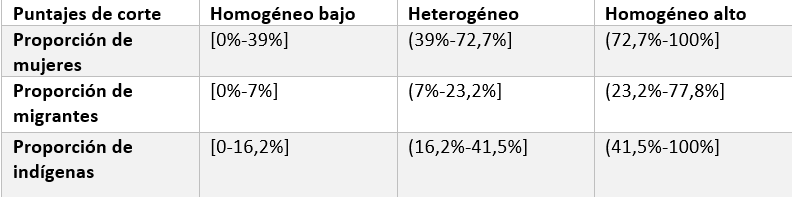
\includegraphics{input/images/puntajes_de_corte.png}

Fuente: Elaboración propia

Tabla 4: Distribución porcentual de establecimientos según grado de
heterogeneidad

\includegraphics{Tesis_files/figure-latex/unnamed-chunk-12-1.pdf}
\includegraphics{Tesis_files/figure-latex/unnamed-chunk-12-2.pdf}
\includegraphics{Tesis_files/figure-latex/unnamed-chunk-12-3.pdf}

Con la información presente en los gráficos de barra, podemos advertir
con precisión, primero, el rango de porcentajes para poder determinar si
cierta proporción de mujeres/indígenas/migrantes en el aula representa
un colegio homogéneo bajo, heterogéneo, u homogéneo alto en la categoría
social correspondiente. Entonces, por ejemplo, un establecimiento que
aloja un 20\% de mujeres sería clasificado como homogéneo bajo (en
términos de género) y un establecimiento con el mismo porcentaje de
migrantes sería catalogado como heterogéneo (en términos
``migratorios'').

Ahora bien, la distribución porcentual según cada variable difere
significativamente por cada atributo social considerado. Mientras en el
caso del sexo de los estudiantes un 74,7\% del total de establecimientos
(que totalizan, en términos absolutos, 2901 como vimos en los
descriptivos) es heterogéneo relativo al género de los estudiantes, sólo
un 19,9\% lo es en relación a la nacionalidad de los alumnos.

\hypertarget{correlaciones}{%
\subsection{Correlaciones}\label{correlaciones}}

\includegraphics{Tesis_files/figure-latex/unnamed-chunk-14-1.pdf}

El gráfico de correlaciones entre variables cuantitativas a nivel
estudiante (ingresos, puntajes SIMCE, y educación) da cuenta de una
asociación alta entre, por un lado, ingreso y educación y, por otro
lado, los puntajes en la prueba SIMCE, particularmente la de Matemática.
En ese caso, las correlaciones son del orden de 0.35 para el caso de
ingresos y 0.36 con la variable educación. Mientras, la correlación
entre estas dos variables cuantitativas y el puntaje en lenguaje es más
baja que la observada en matemáticas, alcanzando el valor de 0.23 para
ingresos y 0.26 para educación. A su vez, se puede apreciar una leve
diferencia en favor de la variable educación.

Las correlaciones entre las dos variables independientes cuantitativas a
nivel estudiante no es lo suficientemente alta como para poder
establecer que están midiendo lo mismo. En consecuencia, está
empiricamente justificado la inclusión de ambas variables en el modelo
por separado.

\hypertarget{gruxe1ficos-bivariados}{%
\subsection{Gráficos bivariados}\label{gruxe1ficos-bivariados}}

\includegraphics{Tesis_files/figure-latex/unnamed-chunk-15-1.pdf}

Si evaluamos el gráfico podremos notar la fuerte asociación existente
entre los puntajes SIMCE y la dependencia administrativa de los
establecimientos escolares. Cada color representa un tipo de dependencia
diferente, donde el rojo es para colegios Municipales, el azul para
colegios subvencionados, y el verde para colegios particulares pagados.
De este modo, existe una jerarquización marcada por puntaje donde
aquellos privados obtienen un mejor rendimiento tanto en matemática como
en lenguaje, mientras aquellos municipales se concentran en la parte más
baja del gráfico. En definitiva, se consolida la idea de que hay una
dependencia contextual de los datos, adicional a las correlaciones
observadas a nivel estudiante en virtud de la varianza que hay en los
puntajes SIMCE entre los diferentes grupos considerados (dependencia
administrativa, ingreso, y educación).

En el caso de los gráficos para el promedio de ingreso por escuela y
promedio educativo, los puntajes de los colegios se asocian
positivamente con estas dos variables. La educación tiene una relación
nítidamente lineal con el promedio SIMCE que tiene cada uno de los
colegios, mientras en el caso de la variable ingreso una función concava
describe de mejor modo el comportamiento de los datos. Por ello, es
esperable que haya un impacto significativo de ambas variables en el
rendimiento de los alumnos, cuya evaluación haremos a partir de la
estimación de los modelos que vienen a continuación.

\hypertarget{modelos}{%
\section{Modelos}\label{modelos}}

\hypertarget{modelo-individual-grupal-y-multinivel}{%
\subsection{Modelo individual, grupal, y
multinivel}\label{modelo-individual-grupal-y-multinivel}}

\usepackage{graphicx}

\begin{table}
\caption{Comparación modelos SIMCE Matemática}
\begin{center}
\scalebox{0.7}{
\begin{tabular}{l c c c}
\hline
 & Individual & Grupal & Multinivel \\
\hline
Intercepto                   & $198.35^{***}$ & $233.80^{***}$ & $179.77^{***}$ \\
                             & $(2.24)$       & $(3.56)$       & $(4.09)$       \\
Ingresos                     & $4.05^{***}$   &                & $3.15^{***}$   \\
                             & $(0.19)$       &                & $(0.19)$       \\
Mujer                        & $-5.45^{***}$  &                & $-5.67^{***}$  \\
                             & $(0.26)$       &                & $(0.26)$       \\
Educación                    & $1.97^{***}$   &                & $1.80^{***}$   \\
                             & $(0.06)$       &                & $(0.06)$       \\
Migrante                     & $3.04^{***}$   &                & $2.94^{***}$   \\
                             & $(0.62)$       &                & $(0.62)$       \\
Indígena                     & $0.09$         &                & $0.33$         \\
                             & $(0.35)$       &                & $(0.35)$       \\
Promedio ingresos            &                & $0.92^{***}$   & $0.82^{***}$   \\
                             &                & $(0.12)$       & $(0.12)$       \\
Heterogeneidad educativa     &                & $3.26^{*}$     & $3.17^{*}$     \\
                             &                & $(1.35)$       & $(1.35)$       \\
Heterogeneidad social        &                & $-0.41^{**}$   & $-0.42^{**}$   \\
                             &                & $(0.15)$       & $(0.15)$       \\
Promedio nivel educativo     &                & $17.44^{***}$  & $15.10^{***}$  \\
                             &                & $(0.85)$       & $(0.85)$       \\
Homogeneidad migratoria alta &                & $-12.72^{***}$ & $-13.26^{***}$ \\
                             &                & $(3.25)$       & $(3.25)$       \\
Homogeneidad migratoria baja &                & $9.05^{***}$   & $9.29^{***}$   \\
                             &                & $(1.34)$       & $(1.34)$       \\
Homogeneidad étnica alta     &                & $7.14^{***}$   & $7.20^{***}$   \\
                             &                & $(2.08)$       & $(2.08)$       \\
Homogeneidad étnica baja     &                & $3.23^{**}$    & $3.24^{**}$    \\
                             &                & $(1.24)$       & $(1.24)$       \\
Alta homogeneidad género     &                & $0.91$         & $3.16$         \\
                             &                & $(2.01)$       & $(2.01)$       \\
Baja homogeneidad género     &                & $-8.53^{***}$  & $-10.07^{***}$ \\
                             &                & $(1.38)$       & $(1.38)$       \\
Particular Subvencionado     &                & $10.31^{***}$  & $10.24^{***}$  \\
                             &                & $(1.36)$       & $(1.36)$       \\
Particular Pagado            &                & $-5.98$        & $-5.60$        \\
                             &                & $(3.75)$       & $(3.75)$       \\
\hline
AIC                          & $1567692.29$   & $1567632.89$   & $1565439.66$   \\
BIC                          & $1567771.52$   & $1567781.46$   & $1565637.76$   \\
Log Likelihood               & $-783838.14$   & $-783801.44$   & $-782699.83$   \\
Num. obs.                    & $147979$       & $147976$       & $147976$       \\
Num. groups: rbd             & $2901$         & $2898$         & $2898$         \\
Var: rbd (Intercept)         & $1593.69$      & $695.73$       & $696.06$       \\
Var: Residual                & $2188.05$      & $2221.70$      & $2188.26$      \\
\hline
\multicolumn{4}{l}{\scriptsize{$^{***}p<0.001$; $^{**}p<0.01$; $^{*}p<0.05$. Errores estándar en paréntesis}}
\end{tabular}
}
\label{table:coefficients}
\end{center}
\end{table}

\pagebreak

En primer lugar, antes de comenzar a describir los párametros de los
modelos estimados, es importante mencionar la cantidad de varianza de
los puntajes de cada una de las pruebas que hay entre las escuelas
chilenas (técnicamente denominada correlación intraclase que se obtiene
a partir del modelo nulo). Siguiendo los resultados, tenemos que un 47\%
de la varianza del puntaje SIMCE Matemática está entre las escuelas.
Para el caso de lenguaje la varianza entre escuelas es más baja, del
orden de 29\%. En consecuencia, se torna pertinente modelar los
resultados en la prueba SIMCE considerando la estructura anidada de los
datos, pues una porción importante de la varianza de los resultados se
explica por la pertenencia a establecimientos escolares.

Si estimamos el modelo de regresión sólo considerando las variables
individuales los datos nos muestran que todas las variables que
teoricamente formulamos como potencialmente explicativas del rendimiento
academico en matemática lo son empiricamente. En ese sentido, todas las
variables incluidas son estadisticamente significativas con un nivel de
confianza equivalente a un 99\%. No obstante, es importante advertir que
el comportamiento de los coeficientes difiere según la prueba SIMCE
considerada.

Las variables que muestran una relación más fuerte con el puntaje SIMCE
de Matematica son, como es esperable, el sexo y los ingresos de los
individuos. El ser mujer está asociado a una pérdida de puntajes del
orden de 5,45 puntos en comparación a lo obtenido por los hombres.
Mientras en el caso de los ingresos tenemos que un incremento del 1\% en
el ingreso per cápita del hogar significa, en promedio, un aumento de
0,04 puntos en la prueba. O, en un sentido más sustantivo, un individuo
que tiene ingresos que ascienden al doble de ingresos que el de otro va
a tener, en promedio, 4,05 puntos más en matemática, manteniendo el
resto de las variables constantes.

Uno de los resultados más contra intuitivos del modelo individual es
que, pese a toda la evidencia acumulada, tanto los indigenas como los
migrantes obtienen mejores resultados que quienes no son indígenas y no
migrantes, respectivamente. De todos modos, el dato más relevante es
aquel referido a nacionalidad cuya significación es muy elevada, pues
tiene un 99,9\% de confianza. Este resultado podría explicarse por la
presencia de migrantes con alto capital cultural y ecónomico, como lo
pueden ser migrantes europeos y estadounidenses, por ejemplo.

En el modelo de regresión que sólo incluye las variables de nivel
escuela, podemos notar que el factor que tiene una mayor influencia en
el rendimiento académico de los colegios es el nivel educativo promedio
de una sala de clases, de modo que el coeficiente asociado a dicha
variable es de 19.82. En efecto, un colegio que tiene un año más de
educación promedio que otro, tendrá una ganancia de puntaje del orden de
20 puntos.

Tanto el promedio de ingreso per cápita del hogar como la desviación
estándar del mismo tienen un efecto muy bajo, y sólo en el caso de la
media es significativo, con un valor bajo de apenas 0,45. Ahora bien, a
partir de los perfiles de establecimientos según el grado de
heterogeneidad existente al interior de ellos podemos determinar el
resultado derivado de cierto contexto o tipo de mixtura social,
cultural, y económica. En ese sentido, en el caso de la nacionalidad,
aquellos colegios con baja concentración de migrantes son los que
obtienen mejor resultado, comparandolo tanto con los establecimientos
heterogéneos como con aquellos que tienen una alta concentración de
migrantes. Asimismo, tiene mejores resultados academicos aquellos
heterogeneos en términos de migrantes que aquellos homogeneos alto en lo
que refiere a la condición migratoria.

En lo que refiere a la composición de género de los establecimientos
escolares, es posible aseverar que aquellos establecimientos que tienen
un mejor rendimiento agregado son aquellos homogeneos alto o bien que
tienen una alta proporción de mujeres en la sala de clases, teniendo
como referencia a aquellos colegios con baja concentración de mujeres.
En último termino, los establecimientos con alta proporción de índigenas
son aquellos que exhiben mejor rendimiento en matemática comparado tanto
con los colegios heterogeneos etnicamente como con los con baja
homogeneidad étnica.

El modelo multinivel, que considera tanto las variables individuales
como las grupales simultaneamente, tiene coeficientes similares a los
obtenidos cuando estimamos los modelos por separado. En esa línea, todos
mantienen su sentido, y su magnitud tiene diferencias casi
imperceptibles.

\begin{table}
\caption{Comparación modelos SIMCE Lenguaje}
\begin{center}
\begin{tabular}{l c c c}
\hline
 & Individual & Grupal & Multinivel \\
\hline
Intercepto                   & $194.43^{***}$ & $236.82^{***}$ & $191.48^{***}$ \\
                             & $(1.97)$       & $(2.67)$       & $(3.23)$       \\
Ingresos                     & $2.80^{***}$   &                & $1.85^{***}$   \\
                             & $(0.17)$       &                & $(0.18)$       \\
Mujer                        & $15.01^{***}$  &                & $14.75^{***}$  \\
                             & $(0.24)$       &                & $(0.24)$       \\
Educación                    & $1.58^{***}$   &                & $1.39^{***}$   \\
                             & $(0.05)$       &                & $(0.05)$       \\
Migrante                     & $1.18^{*}$     &                & $1.18^{*}$     \\
                             & $(0.57)$       &                & $(0.57)$       \\
Indígena                     & $0.22$         &                & $0.46$         \\
                             & $(0.32)$       &                & $(0.32)$       \\
Promedio ingresos            &                & $0.48^{***}$   & $0.42^{***}$   \\
                             &                & $(0.09)$       & $(0.09)$       \\
Heterogeneidad educativa     &                & $1.96$         & $1.80$         \\
                             &                & $(1.02)$       & $(1.01)$       \\
Heterogeneidad social        &                & $-0.33^{**}$   & $-0.32^{**}$   \\
                             &                & $(0.11)$       & $(0.11)$       \\
Promedio nivel educativo     &                & $10.57^{***}$  & $8.74^{***}$   \\
                             &                & $(0.64)$       & $(0.63)$       \\
Homogeneidad migratoria alta &                & $-7.63^{**}$   & $-8.03^{***}$  \\
                             &                & $(2.42)$       & $(2.41)$       \\
Homogeneidad migratoria baja &                & $7.31^{***}$   & $7.34^{***}$   \\
                             &                & $(0.99)$       & $(0.99)$       \\
Homogeneidad étnica alta     &                & $6.10^{***}$   & $6.03^{***}$   \\
                             &                & $(1.53)$       & $(1.53)$       \\
Homogeneidad étnica baja     &                & $1.30$         & $1.52$         \\
                             &                & $(0.91)$       & $(0.91)$       \\
Alta homogeneidad género     &                & $8.08^{***}$   & $2.32$         \\
                             &                & $(1.49)$       & $(1.48)$       \\
Baja homogeneidad género     &                & $-11.06^{***}$ & $-6.93^{***}$  \\
                             &                & $(1.02)$       & $(1.02)$       \\
Particular Subvencionado     &                & $4.42^{***}$   & $4.30^{***}$   \\
                             &                & $(1.00)$       & $(1.00)$       \\
Particular Pagado            &                & $-5.50^{*}$    & $-5.16$        \\
                             &                & $(2.80)$       & $(2.79)$       \\
\hline
AIC                          & $1540411.99$   & $1543577.15$   & $1539097.85$   \\
BIC                          & $1540491.23$   & $1543725.73$   & $1539295.95$   \\
Log Likelihood               & $-770197.99$   & $-771773.58$   & $-769528.93$   \\
Num. obs.                    & $147979$       & $147976$       & $147976$       \\
Num. groups: rbd             & $2901$         & $2898$         & $2898$         \\
Var: rbd (Intercept)         & $586.55$       & $356.54$       & $354.35$       \\
Var: Residual                & $1847.30$      & $1904.94$      & $1847.24$      \\
\hline
\multicolumn{4}{l}{\scriptsize{$^{***}p<0.001$; $^{**}p<0.01$; $^{*}p<0.05$. Errores estándar en paréntesis}}
\end{tabular}
\label{table:coefficients}
\end{center}
\end{table}

En el caso de la prueba SIMCE de lenguaje, hay algunas diferencias
considerables atendiendo a los párametros estimados. Uno de los
elementos más distinguidos de los regresores es que el ser mujer, a
diferencia de lo que ocurría en matemática, está asociado a una ganancia
de puntaje SIMCE, teniendo como categoría de referencia a los hombres. A
su vez, al igual que en matemática, la heterogeneidad en los ingresos de
las familias tiene un impacto negativo en el puntaje SIMCE, contrario a
la hipótesis formulada. Respecto de nuestras variables independientes a
nivel establecimiento escolar ligadas a los perfiles de
establecimientos, tenemos algo similar a lo observado en los modelos de
regresión estimados para la prueba de Mátematica.

Los colegios con alta proporción de mujeres siguen teniendo mejor
rendimiento que los heterogeneos y que los poco homogéneos (o baja
proporción de mujeres en la sala de clases). En el caso de los
establecimientos agrupados segun el nivel de heterogeneidad migratoria,
los datos nos muestran que los que obtienen mejores resultados son
aquellas con baja concentración de migrantes (u homogéneos bajo usando
la jerga habitual). Para efecto del tipo de composición étnica de los
colegios, los modelos son claros en exhibir que aquellos colegios con
alta concentración de indígenas son los mejor evaluados comparado tanto
con establecimientos heterogeneos etnicamente hablando como homogéneo
bajo.

\hypertarget{modelos-multinivel-con-interacciuxf3n-entre-niveles}{%
\subsection{Modelos multinivel con interacción entre
niveles}\label{modelos-multinivel-con-interacciuxf3n-entre-niveles}}

En la siguiente sección procederemos a evaluar si es que existe algún
efecto adicional de los tipos de composición social por pertenecer a
algún género, etnia, y nacionalidad. Concretamente, siguiendo las
hipótesis de investigación contrastaremos tres aseveraciones empíricas
contenidas en ellas. En primer lugar, evaluaremos si la composición de
género de los establecimientos tiene un efecto diferente en las mujeres;
en segundo lugar, si la composición étnica de las escuelas afecta de
modo diferenciado a estudiantes índigenas; y, por último, si acaso la
composición migratoria de los colegios tiene algún tipo de efecto
adicional en la población migrante. Es importante recordar que en los
modelos de regresión ya estimados sólo contrastamos la idea de si la
composición social (en los tres tipos considerados) afecta el
rendimiento acádemico de los alumnos sin distinguir si el efecto era
diferente para las mujeres, índigenas, y migrantes.

\hypertarget{interacciuxf3n-entre-composiciuxf3n-socioecuxf3nomica-y-nivel-socioeconuxf3mico-bajo}{%
\subsubsection{Interacción entre composición socioecónomica y nivel
socioeconómico
bajo}\label{interacciuxf3n-entre-composiciuxf3n-socioecuxf3nomica-y-nivel-socioeconuxf3mico-bajo}}

\includegraphics{Tesis_files/figure-latex/unnamed-chunk-26-1.pdf}
\includegraphics{Tesis_files/figure-latex/unnamed-chunk-26-2.pdf}

Como vimos en los modelos de regresión tanto para lenguaje como
matemática, el efecto de la heterogeneidad socioecónomica de los
colegios medido según el ingreso per cápita del hogar es negativo. Con
ello, se refuta la hipótesis propuesta acerca del efecto positivo que
proyectabamos tenía esta, no obstante, si hacemos interactuar dicha
variable con el nivel socioeconómico de los estudiantes (que la
ingresamos como dicotómica para comparar los dos quintiles más pobres
con los tres más ricos, siendo 0 los primeros y 1 los segundos) resulta
que se modera el efecto negativo de la heterogeneidad para el caso de
los más pobres. En otras palabras, sabiendo que la heterogeneidad es
negativa, esta es menos perjudicial para los alumnos más pobres.

Ahora bien, complementando este resultado, el promedio del nivel
socioeconomico de los colegios tiene consecuencias positivas sobre el
rendimiento tanto en matemática como en lenguaje. Aún más, si la hacemos
interactuar con el nivel socioeconómico de los estudiantes, podremos
apreciar que los más pobres se ven más beneficiados que los más ricos
(comparativamente hablando, pues son los tres quintiles con más
ingresos) a medida que el nivel de ingreso promedio del colegio es más
alto, en términos del puntaje que tienen en la prueba tanto de
matemática como de lenguaje. Si examinamos el gráfico, vemos que la
recta predicha para el nivel socioeconómico bajo tiene una pendiente más
alta comparado con la recta predicha para los individuos de nivel
socioeconómico más alto, dando cuenta de un efecto diferenciado del
promedio socioeconómico de la sala de clases según el origen social del
individuo.

Teniendo a la vista estos datos, cabe preguntarse entonces qué tipo de
configuración de los establecimientos escolares es más deseable en lo
que respecta a su composición socioecónomica. Por un lado, los datos nos
inducen a pensar que una mayor heterogeneidad de los establecimientos
genera un efecto agregado perjudicial sobre el rendimiento de los
estudiantes. Por otro, los estudiantes más pobres mejoran más su
rendimiento que los alumnos no pobres a medida que el contexto
socioecónomico del colegio es más favorable. Ante esta ambivalencia, no
es claro la forma en la que se debiesen distribuir los alumnos en el
sistema educacional, sólo pensando en maximizar el rendimiento académico
de ellos.

\hypertarget{interacciuxf3n-entre-composiciuxf3n-de-guxe9nero-y-sexo}{%
\subsubsection{Interacción entre composición de género y
sexo}\label{interacciuxf3n-entre-composiciuxf3n-de-guxe9nero-y-sexo}}

\begin{table}
\caption{Comparación modelos con interacción sexo/composición género}
\begin{center}
\begin{tabular}{l c c}
\hline
 & Modelo SIMCE Matemática & Modelo SIMCE Lenguaje \\
\hline
Intercepto                       & $179.69^{***}$ & $191.45^{***}$ \\
                                 & $(4.09)$       & $(3.23)$       \\
Ingresos                         & $3.15^{***}$   & $1.85^{***}$   \\
                                 & $(0.19)$       & $(0.18)$       \\
Mujer                            & $-5.52^{***}$  & $14.82^{***}$  \\
                                 & $(0.28)$       & $(0.26)$       \\
Educación                        & $1.80^{***}$   & $1.39^{***}$   \\
                                 & $(0.06)$       & $(0.05)$       \\
Migrante                         & $2.94^{***}$   & $1.18^{*}$     \\
                                 & $(0.62)$       & $(0.57)$       \\
Indígena                         & $0.33$         & $0.46$         \\
                                 & $(0.35)$       & $(0.32)$       \\
Heterogeneidad social            & $-0.42^{**}$   & $-0.32^{**}$   \\
                                 & $(0.15)$       & $(0.11)$       \\
Promedio nivel educativo         & $15.10^{***}$  & $8.74^{***}$   \\
                                 & $(0.85)$       & $(0.63)$       \\
Heterogeneidad educativa         & $3.17^{*}$     & $1.80$         \\
                                 & $(1.35)$       & $(1.01)$       \\
Promedio ingresos                & $0.82^{***}$   & $0.42^{***}$   \\
                                 & $(0.12)$       & $(0.09)$       \\
Homogeneidad migratoria alta     & $-13.25^{***}$ & $-8.03^{***}$  \\
                                 & $(3.25)$       & $(2.41)$       \\
Homogeneidad migratoria baja     & $9.29^{***}$   & $7.34^{***}$   \\
                                 & $(1.34)$       & $(0.99)$       \\
Homogeneidad étnica alta         & $7.20^{***}$   & $6.03^{***}$   \\
                                 & $(2.08)$       & $(1.53)$       \\
Homogeneidad étnica baja         & $3.24^{**}$    & $1.52$         \\
                                 & $(1.24)$       & $(0.91)$       \\
Particular Subvecionado          & $10.24^{***}$  & $4.30^{***}$   \\
                                 & $(1.36)$       & $(1.00)$       \\
Particular Pagado                & $-5.60$        & $-5.16$        \\
                                 & $(3.74)$       & $(2.79)$       \\
Alta homogeneidad género         & $3.85$         & $2.42$         \\
                                 & $(2.75)$       & $(2.27)$       \\
Baja homogeneidad género         & $-9.69^{***}$  & $-6.77^{***}$  \\
                                 & $(1.40)$       & $(1.04)$       \\
Interacción mujer homogéneo alto & $-0.81$        & $-0.14$        \\
                                 & $(2.05)$       & $(1.87)$       \\
Interacción mujer homogéneo bajo & $-1.31$        & $-0.58$        \\
                                 & $(0.85)$       & $(0.78)$       \\
\hline
AIC                              & $1565436.42$   & $1539096.87$   \\
BIC                              & $1565654.32$   & $1539314.77$   \\
Log Likelihood                   & $-782696.21$   & $-769526.43$   \\
Num. obs.                        & $147976$       & $147976$       \\
Num. groups: rbd                 & $2898$         & $2898$         \\
Var: rbd (Intercept)             & $695.87$       & $354.30$       \\
Var: Residual                    & $2188.26$      & $1847.26$      \\
\hline
\multicolumn{3}{l}{\scriptsize{$^{***}p<0.001$; $^{**}p<0.01$; $^{*}p<0.05$. Errores estándar en paréntesis}}
\end{tabular}
\label{table:coefficients}
\end{center}
\end{table}

Según lo discutido en el análisis de los modelos
individual/grupal/multinivel se demostró que, de modo general, aquellos
establecimientos con una alta proporción de mujeres tienen un mejor
rendimiento académico en ambas pruebas SIMCE. Pero, con esa
especificación de los modelos no es posible saber si hay un efecto
diferenciado de dicha composición de género dependiendo del sexo de los
estudiantes. En virtud de ello, estimamos modelos de regresión con
interacción entre niveles, particularmente, entre los perfiles de
establecimiento según género y el sexo de los alumnos.

Los resultados muestran, tanto para la prueba de matemática como de
lenguaje, que el efecto de estar en un colegio heterogéneo para las
mujeres es levemente mayor que para los hombres. Sin embargo, el efecto
de un establecimiento con alta proporción de mujeres es un poco mayor
para los hombres que para las mujeres (sabiendo que, a nivel agregado,
es positivo para los dos) cuando los comparamos con un colegio
heterogéneo.

En resumen, es casi nula la diferencia del efecto de composición de
género según el sexo de los alumnos, lo cual se ve respaldado en que
ninguno de los coeficientes asociados a la interacción entre estas
variables resulta ser significativo. Pese a ello, se confirma la
hipótesis acerca de la relación entre la composición de género y el
rendimiento de las mujeres, pues tanto a ellas como a los hombres les va
mejor, en promedio, con una alta proporción de las primeras en el aula.

\hypertarget{interacciuxf3n-entre-composiciuxf3n-uxe9tnica-e-indigenas}{%
\subsubsection{Interacción entre composición étnica e
indigenas}\label{interacciuxf3n-entre-composiciuxf3n-uxe9tnica-e-indigenas}}

\begin{table}
\caption{Comparación modelos con interacción indígena/composición étnica}
\begin{center}
\begin{tabular}{l c c}
\hline
 & Modelo SIMCE Matemática & Modelo SIMCE Lenguaje \\
\hline
Intercepto                          & $179.78^{***}$ & $191.50^{***}$ \\
                                    & $(4.09)$       & $(3.24)$       \\
Ingresos                            & $3.15^{***}$   & $1.85^{***}$   \\
                                    & $(0.19)$       & $(0.18)$       \\
Mujer                               & $-5.68^{***}$  & $14.75^{***}$  \\
                                    & $(0.26)$       & $(0.24)$       \\
Educación                           & $1.80^{***}$   & $1.39^{***}$   \\
                                    & $(0.06)$       & $(0.05)$       \\
Migrante                            & $2.93^{***}$   & $1.17^{*}$     \\
                                    & $(0.62)$       & $(0.57)$       \\
Indígena                            & $0.18$         & $0.37$         \\
                                    & $(0.54)$       & $(0.49)$       \\
Heterogeneidad social               & $-0.42^{**}$   & $-0.32^{**}$   \\
                                    & $(0.15)$       & $(0.11)$       \\
Promedio nivel educativo            & $15.11^{***}$  & $8.74^{***}$   \\
                                    & $(0.85)$       & $(0.63)$       \\
Heterogeneidad educativa            & $3.17^{*}$     & $1.80$         \\
                                    & $(1.35)$       & $(1.01)$       \\
Promedio ingresos                   & $0.82^{***}$   & $0.42^{***}$   \\
                                    & $(0.12)$       & $(0.09)$       \\
Homogeneidad migratoria alta        & $-13.26^{***}$ & $-8.03^{***}$  \\
                                    & $(3.25)$       & $(2.41)$       \\
Homogeneidad migratoria baja        & $9.29^{***}$   & $7.34^{***}$   \\
                                    & $(1.34)$       & $(0.99)$       \\
Alta homogeneidad género            & $3.16$         & $2.32$         \\
                                    & $(2.01)$       & $(1.48)$       \\
Baja homogeneidad género            & $-10.07^{***}$ & $-6.93^{***}$  \\
                                    & $(1.38)$       & $(1.02)$       \\
Particular Subvencionado            & $10.24^{***}$  & $4.30^{***}$   \\
                                    & $(1.36)$       & $(1.00)$       \\
Particular Pagado                   & $-5.61$        & $-5.16$        \\
                                    & $(3.75)$       & $(2.79)$       \\
Homogeneidad étnica alta            & $6.84^{**}$    & $5.89^{***}$   \\
                                    & $(2.13)$       & $(1.59)$       \\
Homogeneidad étnica baja            & $3.21^{**}$    & $1.50$         \\
                                    & $(1.25)$       & $(0.92)$       \\
Interacción indígena homogéneo alto & $0.73$         & $0.29$         \\
                                    & $(0.98)$       & $(0.90)$       \\
Interacción indígena homogéneo bajo & $0.03$         & $0.09$         \\
                                    & $(0.77)$       & $(0.71)$       \\
\hline
AIC                                 & $1565440.09$   & $1539099.13$   \\
BIC                                 & $1565657.99$   & $1539317.04$   \\
Log Likelihood                      & $-782698.04$   & $-769527.57$   \\
Num. obs.                           & $147976$       & $147976$       \\
Num. groups: rbd                    & $2898$         & $2898$         \\
Var: rbd (Intercept)                & $696.05$       & $354.35$       \\
Var: Residual                       & $2188.28$      & $1847.26$      \\
\hline
\multicolumn{3}{l}{\scriptsize{$^{***}p<0.001$; $^{**}p<0.01$; $^{*}p<0.05$. Errores estándar en paréntesis}}
\end{tabular}
\label{table:coefficients}
\end{center}
\end{table}

La interacción entre la composición étnica y el origen étnico de los
estudiantes arroja que hay un efecto adicional para los indigenas cuando
se encuentran en colegios con alta proporción de su endogrupo en
comparación a los resultados que obtienen cuando están en colegios
heterogeneos étnicamente o de baja homogeneidad étnica. No obstante, los
coeficientes relativos a la interacción entre estas dos variables
alcanza un valor nimio y, por ello, no tiene significación estadística.

De esta forma, si bien a la luz de los resultados empíricos aquí
obtenidos sabemos que los colegios con alta proporción étnica (u
homogeneidad étnica alta) tienen un efecto positivo y significativo en
comparación a los heterogeneos y con baja homogeneidad étnica en ambas
pruebas SIMCE, el efecto en cuestión no difiere significativamente si se
trata de un índigena o no.

\hypertarget{interacciuxf3n-entre-composiciuxf3n-migratoria-y-migrantes}{%
\subsubsection{Interacción entre composición migratoria y
migrantes}\label{interacciuxf3n-entre-composiciuxf3n-migratoria-y-migrantes}}

\begin{table}
\caption{Comparación modelos con interacción migrante/composición migratoria}
\begin{center}
\begin{tabular}{l c c}
\hline
 & Modelo SIMCE Matemática & Modelo SIMCE Lenguaje \\
\hline
Intercepto                          & $179.73^{***}$ & $191.51^{***}$ \\
                                    & $(4.09)$       & $(3.24)$       \\
Ingresos                            & $3.15^{***}$   & $1.85^{***}$   \\
                                    & $(0.19)$       & $(0.18)$       \\
Mujer                               & $-5.67^{***}$  & $14.75^{***}$  \\
                                    & $(0.26)$       & $(0.24)$       \\
Educación                           & $1.80^{***}$   & $1.39^{***}$   \\
                                    & $(0.06)$       & $(0.05)$       \\
Migrante                            & $3.30^{***}$   & $0.95$         \\
                                    & $(0.88)$       & $(0.81)$       \\
Indígena                            & $0.33$         & $0.46$         \\
                                    & $(0.35)$       & $(0.32)$       \\
Heterogeneidad social               & $-0.42^{**}$   & $-0.32^{**}$   \\
                                    & $(0.15)$       & $(0.11)$       \\
Promedio nivel educativo            & $15.10^{***}$  & $8.74^{***}$   \\
                                    & $(0.85)$       & $(0.63)$       \\
Heterogeneidad educativa            & $3.17^{*}$     & $1.80$         \\
                                    & $(1.35)$       & $(1.01)$       \\
Promedio ingresos                   & $0.82^{***}$   & $0.42^{***}$   \\
                                    & $(0.12)$       & $(0.09)$       \\
Homogeneidad étnica alta            & $7.20^{***}$   & $6.03^{***}$   \\
                                    & $(2.08)$       & $(1.53)$       \\
Homogeneidad étnica baja            & $3.24^{**}$    & $1.52$         \\
                                    & $(1.24)$       & $(0.91)$       \\
Alta homogeneidad género            & $3.16$         & $2.32$         \\
                                    & $(2.01)$       & $(1.48)$       \\
Baja homogeneidad género            & $-10.07^{***}$ & $-6.93^{***}$  \\
                                    & $(1.38)$       & $(1.02)$       \\
Particular Subvencionado            & $10.24^{***}$  & $4.30^{***}$   \\
                                    & $(1.36)$       & $(1.00)$       \\
Particular Pagado                   & $-5.61$        & $-5.16$        \\
                                    & $(3.75)$       & $(2.79)$       \\
Homogeneidad migratoria alta        & $-13.04^{***}$ & $-8.05^{**}$   \\
                                    & $(3.31)$       & $(2.48)$       \\
Homogeneidad migratoria baja        & $9.34^{***}$   & $7.31^{***}$   \\
                                    & $(1.35)$       & $(0.99)$       \\
Interacción migrante homogéneo alto & $-0.87$        & $0.20$         \\
                                    & $(2.01)$       & $(1.85)$       \\
Interacción migrante homogéneo bajo & $-0.65$        & $0.51$         \\
                                    & $(1.32)$       & $(1.21)$       \\
\hline
AIC                                 & $1565437.79$   & $1539096.47$   \\
BIC                                 & $1565655.70$   & $1539314.38$   \\
Log Likelihood                      & $-782696.90$   & $-769526.24$   \\
Num. obs.                           & $147976$       & $147976$       \\
Num. groups: rbd                    & $2898$         & $2898$         \\
Var: rbd (Intercept)                & $696.06$       & $354.36$       \\
Var: Residual                       & $2188.28$      & $1847.26$      \\
\hline
\multicolumn{3}{l}{\scriptsize{$^{***}p<0.001$; $^{**}p<0.01$; $^{*}p<0.05$. Errores estándar en paréntesis}}
\end{tabular}
\label{table:coefficients}
\end{center}
\end{table}

Por último, acerca de la interacción entre la composición migratoria y
el estatuto migratorio de los individuos podemos aseverar que las
estimaciones nos proporcionan resultados diferentes en función de la
prueba SIMCE considerada. Si evaluamos la interacción para la prueba de
lenguaje, el efecto adicional de pertenecer a una escuela heterogenea en
términos de nacionalidad para los migrantes es negativa. Por el
contrario, los migrantes que son parte de escuelas heterogéneas en
términos de su composición migratoria tienen un puntaje adicional
positivo en comparación a lo obtenido en colegios homogéneos.

Pese a lo anterior, es importante subrayar que los coeficientes
asociados a la interacciones estimadas no son significativos
estadísticamente, razón por la cual la interpretación aquí ofrecida sólo
tiene sentido a nivel muestral (que, por cierto, se parece a la
población por tratarse de una muestra muy grande).

\hypertarget{discusiuxf3n-de-los-resultados}{%
\section{Discusión de los
resultados}\label{discusiuxf3n-de-los-resultados}}

\hypertarget{retomando-las-hipuxf3tesis-de-investigaciuxf3n}{%
\subsection{Retomando las hipótesis de
investigación}\label{retomando-las-hipuxf3tesis-de-investigaciuxf3n}}

La discusión acerca del fenómeno de la segregación social y, más
especificamente, de la composición de los establecimientos escolares es
fundamental en nuestro país, cuyo contexto educativo exhibe altos
niveles de discriminación, estratificación, y segmentación sociocultural
de sus estudiantes. En estas circunstancias, nos preguntamos por la
relación que hay en el sistema educacional chileno entre, por un lado,
el grado de heterogeneidad de la composición escolar y los resultados en
la prueba SIMCE de matemática y lenguaje.

Siguiendo dicho objetivo, formulamos tres hipótesis que procuraban
recoger los debates en la literatura nacional e internacional sobre el
tópico de composición. En primer lugar, acerca del nivel socioeconómico
se planteó que mayores niveles de heterogeneidad socioeconómica tendrían
un efecto positivo en el conjunto de los estudiantes y que además, iba a
tener un efecto positivo adicional en la población más pobre comparada
con aquella que tiene más ingresos.

Los resultados empíricos obtenidos nos permiten rechazar parcialmente la
hipótesis. Si bien el efecto de la heterogeneidad socioecónomica era
negativo, este se hacía menos negativo o se veía moderado en los
estudiantes más pobres. Asimismo, se mostró gráficamente, que los
estudiantes de niveles socioecónomicos más bajos se ven mucho más
beneficiados de niveles promedio de ingreso elevado de la sala de clases
que aquellos sectores de origen socioeconómico más alto. En vistas de
estos resultados, se vuelve complejo dirimir el debate acerca de la
mixtura social, al menos en su dimensión socioecónomica.

Por una parte, si los alumnos más pobres se cambian a escuelas de
mayores niveles de ingreso, ciñiendonos por las predicciones de los
modelos, debiesen tener una ganancia de puntaje. Por otra parte, dicha
escuela se haría más heterogénea y, con ello, tal como se establece en
la estimación, habría un efecto negativo sobre esos mismos estudiantes.

Acerca de nuestra segunda hipótesis, relativa a la composición de género
y el rendmiento de las mujeres, los modelos estimados son claros en
mostrar que tanto estudiantes hombres como mujeres obtienen un
rendimiento ostensiblemente superior cuando se encuentran en colegios
homogéneos con alta concentración de mujeres, en comparación a lo
obtenido en uno heterogéneo o de baja homogeneidad. Adicionalmente,
cuando contrastamos la posibilidad de que dicho efecto fuese más fuerte
en mujeres que en los hombres nos encontramos con que en el caso de un
colegio heterogéneo comparado con cualquiera de los homogéneos ocurría
así, mientras que en el caso de uno homogéneo con alta proporción de
mujeres el efecto positivo se hacía más positivo en hombres que en
mujeres. De todos modos, las diferencias eran muy pequeñas y no
significativas, razón por la cual el resultado más robusto es aquel
referido al primer efecto descrito.

En tercer lugar, la hipótesis propuesta en materia étnica y migrante
consistente en que una mayor heterogeneidad étnica, para el caso de los
indígenas, y migratoria para el caso de los migrantes sería mejor que un
ambiente homogéneo en estas dimensiones considerando los resultados
académicos, es parcialmente cierto.

En ese sentido, aquellos establecimientos con baja concentración de
migrantes (u homogéneo bajo) tienen puntuaciones más altas tanto en
matemática como en lenguaje comparado con colegios heterogéneos, no
obstante, aquellos establecimientos heterogéneos tienen un mejor
rendimiento comparado con aquellos homogéneos alto. En virtud de ello,
se puede sostener que tanto para los migrantes como para los nacionales
es mejor pertenecer a un colegio heterogéneo según nacionalidad que uno
en el cual haya una alta concentración de migrantes.

En la misma línea, en el caso de la composición étnica de las escuelas
los resultados son diferentes. Las escuelas heterogéneas obtienen peores
resultados comparado con los dos perfiles de homogeneidad étnica (alta y
baja) lo cual contraviene directamente lo propuesto acerca de la
composición étnica en la tercera hipótesis. De todos modos, cabe
subrayar que las escuelas con alta concentración de indígenas puntúan
más en las dos pruebas que las con baja concentración de estudiantes de
origen indígena.

Desde una perspectiva de política educacional, los productos aquí
obtenidos nos permiten consignar algunas orientaciones a la vez que
constatar ambieguedades y nudos irresueltos que deben permanecer en
constante estudio. Uno de los principales puntos que se desmitifica es
que la mixtura social y cultural resulta ser completamente perjudicial.
Según los hallazgos, en muchos casos un contexto más heterogéneo es más
conveniente que uno homogéneo (tal es el caso para los migrantes y, con
alguna salvedad, para los quintiles más pobres) evaluado según el
rendimiento académico.

Asimismo, un resultado que confirma la hipótesis de trabajo pero que no
está exento de polémicas es el caso de la composición de género. Los
resultados nos indican que aquellos establecimientos con una alta
proporción de mujeres muestran mejores resultados que aquellos
heterogéneos y aquellos con baja homogeneidad. Entonces, la pregunta que
emerge a partir de lo anterior es si los colegios se debiesen separar
por género en virtud de los mejores resultados mostrados por los
colegios con alta cantidad de mujeres. Sabiendo los múltiples beneficios
típicos de una educación mixta (citar acá), sumado a que es un proceso
muy extendido (sólo un porcentaje muy bajo de colegios abarca
estudiantes de un sólo género) se debiese incursionar en las causas y
mecanismos que explican que un contexto educativo con esa composición de
género sea más favorable que las otras, en relación con el rendimiento
académico.

Por último, la relación del contexto socioeconómico de la sala de clases
y el rendimiento de los alumnos más pobres es difusa. Aun cuando la
heterogeneidad socioeconómica del colegio impacta negativamente en el
rendimiento académico de los estudiantes, los estudiantes más pobres se
ven más beneficiados, considerablmente, de establecimientos escolares
con un nivel de ingreso más alto. De esta forma, no es claro si es
conveniente, desde una perspectiva descriptiva (es decir, sólo
decidiendo a partir de los resultados empíricos exhibidos en SIMCE), una
mayor mixtura al interior de los colegios.

\hypertarget{limitaciones-del-estudio}{%
\subsection{Limitaciones del estudio}\label{limitaciones-del-estudio}}

La investigación desarrollada tiene varias limitaciones sumamente
relevante de mencionar y a corregir en investigaciones futuras. En
primer lugar, los datos con los que se trabajan podrían tener un sesgo
significativo en la medida que sólo se trabaja con 148 mil
(aproximadamente) de los 270 mil alumnos que rindieron el SIMCE de II
medio el año 2017. De todas formas, el tamaño de la muestra alcanzada es
grande y, también, la distribución empírica de algunas variables (por
ejemplo del ingreso per cápita) se asemeja a lo que ocurre efectivamente
en la población chilena (dando luces de que dicho sesgo bien podría ser
inexistente).

En segundo lugar, el enfoque metodológico de la investigación es de
cáracter transversal lo cual, necesariamente, implica ciertas
limitaciones. En consecuencia, no es admisible descartar que el
comportamiento observado de los datos se explique por alguna(s)
variable(s) de orden longitudinal (por ejemplo, el rendimiento previo de
los estudiantes).

En tercer lugar, es posible que hayan variables fundamentales no
incluidas que puedan estar muy vinculadas al rendimiento académico de
los alumnos. El fenómeno educacional es de gran complejidad, lo cual
implica que, al momento de modelar dicho fenómeno, siempre se dejan
fuera elementos, componentes, y dimensiones que subyacen a esta
problemática.

En cuarto lugar, la forma de construcción del nivel socioecónomico se
hizo sólo a partir de los ingresos, pues nos encontramos delimitados por
los datos que no tenían más preguntas de caracterización socioecónomica
que hubiesen servido para medir de manera más multidimensional dicho
constructo.

\hypertarget{investigaciones-futuras}{%
\subsection{Investigaciones futuras}\label{investigaciones-futuras}}

La investigación desarrollada significa una contribución importante en
materia de composición escolar y la relación que tiene sus distintas
formas de distribución en el rendimiento acádemico. No obstante, el
proceso educativo no sólo abarca el cultivo de aptitudes cognitivas de
los estudiantes. Por ello, investigaciones futuras debiesen evaluar la
relación del fenomeno de la composición escolar con el ambiente generado
en la sala, la motivación de los estudiantes, y el desarrollo
psicosocial de los alumnos. En medio de un escenario educativo de
fragmentación ecónomica, social, y cultural, es fundamental conocer los
impactos que ello tiene en la formación de los estudiantes chilenos.

El enfoque con el cual nos aproximamos al tópico investigado tuvo más
bien un cáracter descriptivo en el sentido de que buscamos cuantificar y
medir empíricamente la relación entre el grado de heterogeneidad de la
composición y el puntaje SIMCE. Sumado a lo anterior, es crucial
explicitar y profundizar en la discusión normativa que intersecta el
estudio de la composición escolar. En ese sentido, no solo cabe
preguntarse por la magnitud de la segregación,
heterogeneidad/homogeneidad de los colegios, sino también ahondar en la
pertinencia o no de un sistema educacional más equitativo, mixto, con
una interacción dinámica entre los diversos grupos sociales y culturales
que son parte de la sociedad chilena.

En esa línea, la reciente (y aún no culminada) implementación de la
nueva ley de eduación pública (que desmunicipaliza la educación pública)
y la ley de inclusión, la cual pone fin a la selección y el copago en
establecimientos subvencionados va en la dirección de propiciar una
mayor equidad social, asentada en la idea de una educación orientada a
cultivar la no discriminación, el trato igualitario entre diversos
géneros, culturas, grupos sociales y, en definitiva, una mayor cohesión
social a nivel del país. Entonces, de algún modo, la tarea para los
investigadores en educación es resguardar un diseño que, por un lado,
garantize efectivmaente mayor igualdad, mixtura y equidad al interior
del sistema educacional y, por otro, sin descuidar los potenciales
efectos negativos que podría tener en los resultados académicos (y
también otras dimensiones no evaluadas en este estudio) que, en cierto
grado, evidenciamos en esta investigación.

Como antecedente fundamental de lo anterior, existe vasta evidencia de
sistemas educacionales con niveles de equidad y mixtura social muy alta
con, al mismo tiempo, resultados sobresalientes en el proceso formativo
de los estudiantes. Tal es el caso de Finlandia, Dinamarca, y muchos
otros países Europeos que se caracterizan por tener una educación
pública extendida y robusta. Con ello, se demuestra que es completamente
posible y factible el desarrollo de un sistema educacional que armonice
niveles altos de igualdad y mixtura social con buenos resultados por
parte de sus estudiantes. Quizás esto último esté vinculado a lo
primero, hipótesis que excede con creces a lo inferible a partir de
nuestros resultados.

Finalmente, destacar la imperiosa necesidad de seguir falseando y
contrastando las hipótesis formulados mediante la inclusión de otras
variables de control que, eventualmente, puedan estar detrás de las
diferencias observadas entre perfiles y interacciones contrastados. Con
ello, se contribuira a precisar el alcance real que tiene la
heterogeneidad de la composicion en los resultados académicos.

\hypertarget{bibliografuxeda}{%
\section*{Bibliografía}\label{bibliografuxeda}}
\addcontentsline{toc}{section}{Bibliografía}

\hypertarget{refs}{}
\leavevmode\hypertarget{ref-agirdag_why_2012}{}%
Agirdag, O., Van Houtte, M., \& Van Avermaet, P. (2012). Why Does the
Ethnic and Socio-economic Composition of Schools Influence Math
Achievement? The Role of Sense of Futility and Futility Culture.
\emph{European Sociological Review}, \emph{28}(3), 366--378.
\url{https://doi.org/10.1093/esr/jcq070}

\leavevmode\hypertarget{ref-alejandrocarrasco_mercado_2016}{}%
Alejandro Carrasco,;. G.-H. (2016). \emph{Mercado escolar: Libertad,
diversidad y desigualdad}.

\leavevmode\hypertarget{ref-angrist_does_2004}{}%
Angrist, J. D., \& Lang, K. (2004). Does School Integration Generate
Peer Effects? Evidence from Boston's Metco Program. \emph{American
Economic Review}, \emph{94}(5), 1613--1634.
\url{https://doi.org/10.1257/0002828043052169}

\leavevmode\hypertarget{ref-arteaga_school_2014}{}%
Arteaga, F., Paredes, V., \& Paredes, R. (2014). School Segregation in
Chile: Residence, Copayment or Preferences? \emph{Unpublished
Manuscript}.

\leavevmode\hypertarget{ref-atria_mala_2012}{}%
Atria, F. (2012). \emph{La mala educación: Ideas que inspiran al
movimiento estudiantil en Chile} (Primera edición). Catalonia : CIPER,
Centro de Investigación Periodística.

\leavevmode\hypertarget{ref-bafalluy_modernizacion_1983}{}%
Bafalluy, A. P. (1983). \emph{La modernización educacional}. Ediciones
Universidad Católica de Chile.

\leavevmode\hypertarget{ref-becker_human_1993}{}%
Becker, G. S. (1993). \emph{Human capital: A theoretical and empirical
analysis, with special reference to education} (3rd ed). The University
of Chicago Press.

\leavevmode\hypertarget{ref-bellei_expansion_2007}{}%
Bellei, C. (2007). Expansión de la educación privada y mejoramiento de
la educación en Chile. Evaluación a partir de la evidencia.
\emph{Pensamiento Educativo}, \emph{40}(1), 285--311.

\leavevmode\hypertarget{ref-bellei_estudio_2013}{}%
Bellei, C. (2013). El estudio de la segregación socioeconómica y
académica de la educación chilena. \emph{Estudios Pedagógicos
(Valdivia)}, \emph{39}(1), 325--345.
\url{https://doi.org/10.4067/S0718-07052013000100019}

\leavevmode\hypertarget{ref-bellei_conocer_2010}{}%
Bellei, C., \& Pérez, V. (2010). \emph{Conocer más para vivir mejor.
Educación y conocimiento en Chile en la perspectiva del Bicentenario}.
Taurus.

\leavevmode\hypertarget{ref-bellei_nueva_2018}{}%
Bellei, Muñoz, G., Rubio, X., \& Alcaino, M. (2018). \emph{La Nueva
Educación Pública. Contexto, contenidos y perspectivas de la
desmunicipalización}. LOM Ediciones.

\leavevmode\hypertarget{ref-bellei_gran_2015}{}%
Belleï, C. (2015). \emph{El gran experimento: Mercado y privatización de
la educación chilena} (Primera edición). LOM Ediciones.

\leavevmode\hypertarget{ref-bertrand_new_2011}{}%
Bertrand, M. (2011). \emph{New Perspectives on Gender} (pp. 1543--1590)
{[}Handbook of Labor Economics{]}. Elsevier.

\leavevmode\hypertarget{ref-bonal_understanding_2019b}{}%
Bonal, X., \& Bellei, C. (Eds.). (2019). \emph{Understanding School
Segregation: Patterns, Causes and Consequences of Spatial Inequalities
in Education}. Bloomsbury Publishing Plc.
\url{https://doi.org/10.5040/9781350033542}

\leavevmode\hypertarget{ref-bone_girls_1983}{}%
Bone, A. (1983). \emph{Girls and Girl-only School: Vol. Manchester:
Equal Opportunities Commission}. \emph{Manchester: Equal Opportunities
Commission}.

\leavevmode\hypertarget{ref-bourdieu_herederos_2009}{}%
Bourdieu, P., \& Passeron, J.-C. (2009). \emph{Los herederos: los
estudiantes y la cultura}. Siglo Veintiuno Editores Argentina.

\leavevmode\hypertarget{ref-bourdieu_reproduccion_1998}{}%
Bourdieu, P., Passeron, J. C., Melendres, J., \& Subirats, M. (1998).
\emph{La reproducción: elementos para una teoría del sistema de
enseñanza}. Distribuciones Fontamara.

\leavevmode\hypertarget{ref-canales_educational_2018}{}%
Canales, A., \& Webb, A. (2018). Educational Achievement of Indigenous
Students in Chile: School Composition and Peer Effects.
\emph{Comparative Education Review}, \emph{62}(2), 231--273.
\url{https://doi.org/10.1086/696957}

\leavevmode\hypertarget{ref-castillo_estudiantes_2018}{}%
Castillo, D., Santa Cruz-Grau, E., \& Vega, A. (2018). Estudiantes
migrantes en escuelas públicas chilenas. \emph{Calidad En La Educación},
\emph{49}, 18. \url{https://doi.org/10.31619/caledu.n49.575}

\leavevmode\hypertarget{ref-cerda_situacion_2009}{}%
Cerda, R. (2009). Situación socioeconómica reciente de los mapuches en
la Región de la Araucanía. \emph{Estudios Públicos}, \emph{113}.
\url{https://doi.org/10.38178/cep.vi113.445}

\leavevmode\hypertarget{ref-coleman_equality_1965}{}%
Coleman, J. (1965). \emph{Equality of Educational Opportunity} (John
Hopkins University).

\leavevmode\hypertarget{ref-contini_immigrant_2013}{}%
Contini, D. (2013). Immigrant background peer effects in Italian
schools. \emph{Social Science Research}, \emph{42}(4), 1122--1142.
\url{https://doi.org/10.1016/j.ssresearch.2013.02.003}

\leavevmode\hypertarget{ref-contreras_when_2010}{}%
Contreras, D., Sepúlveda, P., \& Bustos, S. (2010). When Schools Are the
Ones that Choose: The Effects of Screening in Chile*: School Vouchers in
Chile. \emph{Social Science Quarterly}, \emph{91}(5), 1349--1368.
\url{https://doi.org/10.1111/j.1540-6237.2010.00735.x}

\leavevmode\hypertarget{ref-driessen_ethnicity_2001}{}%
Driessen, G. W. J. M. (2001). Ethnicity, Forms of Capital, and
Educational Achievement. \emph{International Review of Education/
Internationale Zeitschrift Fr Erziehungswissenschaft/ Revue Inter},
\emph{47}(6), 513--538. \url{https://doi.org/10.1023/A:1013132009177}

\leavevmode\hypertarget{ref-dronkers_school_2007}{}%
Dronkers, J., \& Levels, M. (2007). Do School Segregation and School
Resources Explain Region-of-Origin Differences in the Mathematics
Achievement of Immigrant Students? \emph{Educational Research and
Evaluation}, \emph{13}(5), 435--462.
\url{https://doi.org/10.1080/13803610701743047}

\leavevmode\hypertarget{ref-dronkers_positive_2013a}{}%
Dronkers, J., \& van der Velden, R. (2013). Positive but also Negative
Effects of Ethnic Diversity in Schools on Educational Performance? An
Empirical Test Using PISA Data. In M. Windzio (Ed.), \emph{Integration
and Inequality in Educational Institutions} (pp. 71--98). Springer
Netherlands. \url{https://doi.org/10.1007/978-94-007-6119-3_4}

\leavevmode\hypertarget{ref-dumay_does_2008}{}%
Dumay, X., \& Dupriez, V. (2008). Does the school composition effect
matter? Evidence from Belgian data. \emph{British Journal of Educational
Studies}, \emph{56}(4), 440--477.
\url{https://doi.org/10.1111/j.1467-8527.2008.00418.x}

\leavevmode\hypertarget{ref-elacqua_impact_2012}{}%
Elacqua, G. (2012). The impact of school choice and public policy on
segregation: Evidence from Chile. \emph{International Journal of
Educational Development}, \emph{32}(3), 444--453.
\url{https://doi.org/10.1016/j.ijedudev.2011.08.003}

\leavevmode\hypertarget{ref-flores_consecuencias_2006}{}%
Flores, C. (2006). \emph{Consecuencias de la segregación residencial:
Teoría y métodos}. 197--230.

\leavevmode\hypertarget{ref-garcia-huidobro_desigualdad_2007}{}%
Garcia-Huidobro, J. (2007). Desigualdad educativa y segmentación del
sistema escolar. Consideraciones a partir del caso chileno. In
\emph{undefined}.
/paper/Desigualdad-educativa-y-segmentaci\%C3\%B3n-del-sistema-a-Garcia-Huidobro/019fba1be198f3223624efad75744f69dfb3b299.

\leavevmode\hypertarget{ref-gonzalez_segregacion_2017}{}%
González, R. (2017). Segregación educativa en el sistema chileno desde
una perspectiva comparada. \emph{Centro de Estudios Del Ministerio de
Educación. Santiago. Chile}.

\leavevmode\hypertarget{ref-gray_estimating_1990}{}%
Gray, J., Jesson, D., \& Sime, N. (1990). Estimating Differences in the
Examination Performances of Secondary Schools in Six LEAs: A multi-level
approach to school effectiveness. \emph{Oxford Review of Education},
\emph{16}(2), 137--158. \url{https://doi.org/10.1080/0305498900160201}

\leavevmode\hypertarget{ref-hannan_coeducation_1996}{}%
Hannan, D., Smyth, E., McCullagh, J., O'Leary, R., \& McMahon, D.
(1996). \emph{Coeducation and Gender Equality: Exam Performance, Stress
and Personal Development}. Oak Tree Press in association with the ESRI.

\leavevmode\hypertarget{ref-hansen_social_1997}{}%
Hansen, M. N. (1997). Social and Economic Inequality in the Educational
Career: Do the Effects of Social Background Characteristics Decline?
\emph{European Sociological Review}, \emph{13}(3), 305--321.
\url{https://doi.org/10.1093/oxfordjournals.esr.a018220}

\leavevmode\hypertarget{ref-harker_effects_2004}{}%
Harker, R., \& Tymms, P. (2004). The Effects of Student Composition on
School Outcomes. \emph{School Effectiveness and School Improvement},
\emph{15}(2), 177--199.
\url{https://doi.org/10.1076/sesi.15.2.177.30432}

\leavevmode\hypertarget{ref-hernandez_eleccion_2015}{}%
Hernández, M., \& Raczynski, D. (2015). Elección de escuela en Chile: De
las dinámicas de distinción y exclusión a la segregación socioeconómica
del sistema escolar. \emph{Estudios Pedagógicos (Valdivia)},
\emph{41}(2), 127--141.
\url{https://doi.org/10.4067/S0718-07052015000200008}

\leavevmode\hypertarget{ref-hoxby_peer_2000}{}%
Hoxby, C. (2000). \emph{Peer Effects in the Classroom: Learning from
Gender and Race Variation} (Working Paper Nos. 7867; Working Paper
Series). National Bureau of Economic Research.
\url{https://doi.org/10.3386/w7867}

\leavevmode\hypertarget{ref-hoxby_taking_2005}{}%
Hoxby, C. M., \& Weingarth, G. (2005). \emph{Taking race out of the
equation: School reassignment and the structure of peer effects}. 44.

\leavevmode\hypertarget{ref-james_measures_1985}{}%
James, D. R., \& Taeuber, K. E. (1985). Measures of Segregation'in NB
Tuma. \emph{Sociological Methodology}.

\leavevmode\hypertarget{ref-jofre1988sistema}{}%
Jofre, G. (1988). \emph{El Sistema de subvenciones en educación: La
experiencia chilena}. Centro de Estudios Publicos.

\leavevmode\hypertarget{ref-koedel_math_2012}{}%
Koedel, C., \& Tyhurst, E. (2012). Math skills and labor-market
outcomes: Evidence from a resume-based field experiment. \emph{Economics
of Education Review}, \emph{31}(1), 131--140.
\url{https://doi.org/10.1016/j.econedurev.2011.09.006}

\leavevmode\hypertarget{ref-mayol_derrumbe_2015}{}%
Mayol, A. (2015). \emph{El derrumbe del modelo: la crisis de la economía
de mercado en el Chile contemporáneo}. LOM Ediciones.

\leavevmode\hypertarget{ref-mcewan_indigenous_2004}{}%
McEwan, P. J. (2004). The Indigenous Test Score Gap in Bolivia and
Chile. \emph{Economic Development and Cultural Change}, \emph{53}(1),
157--190.

\leavevmode\hypertarget{ref-mcewan_can_2008}{}%
McEwan, P. J. (2008). Can Schools Reduce the Indigenous Test Score Gap?
Evidence from Chile. \emph{The Journal of Development Studies},
\emph{44}(10), 1506--1530.
\url{https://doi.org/10.1080/00220380802265223}

\leavevmode\hypertarget{ref-merry_equality_2012}{}%
Merry, M. S., \& Driessen, G. (2012). Equality on Different Terms: The
Case of Dutch Hindu Schools. \emph{Education and Urban Society},
\emph{44}(5), 632--648. \url{https://doi.org/10.1177/0013124511404887}

\leavevmode\hypertarget{ref-mizala_bringing_2012}{}%
Mizala, A., \& Torche, F. (2012). Bringing the schools back in: The
stratification of educational achievement in the Chilean voucher system.
\emph{International Journal of Educational Development}, \emph{32}(1),
132--144. \url{https://doi.org/10.1016/j.ijedudev.2010.09.004}

\leavevmode\hypertarget{ref-murillo_evolucion_2018}{}%
Murillo, F. J., Duk, C., \& Garrido, C. M. (2018). Evolución de la
segregación socioeconómica de las escuelas de América Latina.
\emph{Estudios Pedagógicos}, \emph{44}(1), 157--179.
\url{https://doi.org/10.4067/S0718-07052018000100157}

\leavevmode\hypertarget{ref-nash_school_2003}{}%
Nash, R. (2003). Is the School Composition Effect Real?: A Discussion
With Evidence From the UK PISA Data. \emph{School Effectiveness and
School Improvement}, \emph{14}(4), 441--457.
\url{https://doi.org/10.1076/sesi.14.4.441.17153}

\leavevmode\hypertarget{ref-nash_progress_1997}{}%
Nash, R., \& Harker, R. K. (1997). \emph{Progress at school: Final
report to the ministry of education}. Wellington: Ministry of Education.

\leavevmode\hypertarget{ref-nunezprieto_educacion_2015}{}%
Nuñez Prieto, I. (2015). Educación chilena en la República: Promesas de
universalismo y realidades de inequidad en su historia.
\emph{Psicoperspectivas}, \emph{14}(3), 5--16.
\url{https://doi.org/10.5027/psicoperspectivas-Vol14-Issue3-fulltext-617}

\leavevmode\hypertarget{ref-nunez_transformaciones_1984}{}%
Núñez, I. (1984). \emph{Las transformaciones educacionales bajo el
Régimen Militar. Programa Interdisciplinario de Investigaciones en
Educación} (Programa Interdisciplinario de Investigaciones en Educación,
PIIE).

\leavevmode\hypertarget{ref-oecd_pisa_2016}{}%
OECD. (2016). \emph{PISA 2015 Results (Volume I): Excellence and Equity
in Education}. OECD. \url{https://doi.org/10.1787/9789264266490-en}

\leavevmode\hypertarget{ref-opdenakker_relationship_2001}{}%
Opdenakker, M.-C., \& Damme, J. (2001). Relationship between School
Composition and Characteristics of School Process and their Effect on
Mathematics Achievement. \emph{British Educational Research Journal},
\emph{27}(4), 407--432. \url{https://doi.org/10.1080/01411920120071434}

\leavevmode\hypertarget{ref-ortega_centrality_2020}{}%
Ortega, L., Boda, Z., Treviño, E., Arriagada, V., Gelber, D., \&
Escribano, M. del R. (2020). The centrality of immigrant students within
teacher-student interaction networks: A relational approach to
educational inclusion. \emph{Teaching and Teacher Education}, \emph{95},
103126. \url{https://doi.org/10.1016/j.tate.2020.103126}

\leavevmode\hypertarget{ref-ortiz_escuelas_2015}{}%
Ortiz, I. (2015). Escuelas inclusivas en el contexto de segregación
social del sistema escolar chileno. \emph{Calidad En La Educación},
\emph{42}, 93--122.
\url{https://doi.org/10.4067/S0718-45652015000100004}

\leavevmode\hypertarget{ref-palet_desiguales_2017}{}%
Palet, A., Aguirre, P. de, \& Chile, P. (Eds.). (2017).
\emph{Desiguales: Orígenes, cambios y desafíos de la brecha social en
Chile}. PNUD : Uqbar Editores.

\leavevmode\hypertarget{ref-paredes_mixed_2018}{}%
Paredes, V. (2018). Mixed but not Scrambled Gender Gaps in Single-Sex
Classrooms. In \emph{Working Papers} (Nos. wp470). University of Chile,
Department of Economics.

\leavevmode\hypertarget{ref-radovicsendra_diferencias_2017}{}%
Radovic Sendra, D. (2017). Diferencias de género en rendimiento
matemático en Chile. \emph{Revista Colombiana de Educación}, \emph{74},
221. \url{https://doi.org/10.17227/rce.num74-6907}

\leavevmode\hypertarget{ref-riedemann_sobre_2015}{}%
Riedemann, A., \& Stefoni, C. (2015). Sobre el racismo, su negación, y
las consecuencias para una educación anti-racista en la enseñanza
secundaria chilena. \emph{Polis (Santiago)}, \emph{14}(42), 191--216.
\url{https://doi.org/10.4067/S0718-65682015000300010}

\leavevmode\hypertarget{ref-sammons_forging_1997}{}%
Sammons, P., Thomas, S. M., \& Mortimore, P. (1997). \emph{Forging
Links: Effective Schools and Effective Departments}.

\leavevmode\hypertarget{ref-smyth_singlesex_2010}{}%
Smyth, E. (2010). Single-sex Education: What Does Research Tell Us?
\emph{Revue Française de Pédagogie}, \emph{171}, 47--58.
\url{https://doi.org/10.4000/rfp.1896}

\leavevmode\hypertarget{ref-szulkin_ethnic_2007}{}%
Szulkin, R., \& Jonsson, J. O. (2007). Ethnic Segregation and
Educational Outcomes in Swedish Comprehensive Schools. In \emph{SULCIS
Working Papers} (2007:2). Stockholm University, Linnaeus Center for
Integration Studies - SULCIS.

\leavevmode\hypertarget{ref-taut_efecto_2012}{}%
Taut, S., \& Escobar, J. (2012). El efecto de las características de los
pares en el aprendizaje de estudiantes chilenos de enseñanza media.
\emph{MINISTERIO DE EDUCACION}.

\leavevmode\hypertarget{ref-thrupp_school_2002b}{}%
Thrupp, M., Lauder, H., \& Robinson, T. (2002). School composition and
peer effects. \emph{International Journal of Educational Research},
\emph{37}(5), 483--504.
\url{https://doi.org/10.1016/S0883-0355(03)00016-8}

\leavevmode\hypertarget{ref-tijoux_escuelas_2013}{}%
Tijoux, M. E. (2013). Las escuelas de la inmigración en la ciudad de
Santiago: Elementos para una educación contra el racismo. \emph{Polis
(Santiago)}, \emph{12}(35), 287--307.
\url{https://doi.org/10.4067/S0718-65682013000200013}

\leavevmode\hypertarget{ref-trevino_educacion_2017}{}%
Treviño, E., Morawietz, L., Villalobos, C., Villalobos, E., \& Centro de
Estudios de Políticas y Prácticas en Educación (Chile) (Eds.). (2017).
\emph{Educación intercultural en Chile: Experiencias, pueblos y
territorios}. Centro UC Estudios de Políticas y Prácticas en
Educación--CEPPE : Ediciones UC.

\leavevmode\hypertarget{ref-trevino_segregacion_2014}{}%
Treviño, E., Valenzuela, J., \& Villalobos, C. (2014). Segregación
académica y socioeconómica al interior de la escuela. Análisis de su
magnitud, evolución y principales factores explicativos. \emph{Fonide}.

\leavevmode\hypertarget{ref-undurraga_unraveling_2014}{}%
Undurraga, E. (2014). \emph{Unraveling Development: Three Essays on
Structural Determinants of Human Capabilities} {[}PhD thesis{]}.
Brandeis University.

\leavevmode\hypertarget{ref-valenzuela_evolucion_2008}{}%
Valenzuela, J. P., Bellei, C., \& De los Rios, D. (2008).
\emph{Evolución de la segregación socioeconómica de los estudiantes
chilenos y su relación con el financiamiento compartido}.

\leavevmode\hypertarget{ref-valenzuela_socioeconomic_2014}{}%
Valenzuela, J. P., Bellei, C., \& Ríos, D. de los. (2014). Socioeconomic
school segregation in a market-oriented educational system. The case of
Chile. \emph{Journal of Education Policy}, \emph{29}(2), 217--241.
\url{https://doi.org/10.1080/02680939.2013.806995}

\leavevmode\hypertarget{ref-vandegaer_effects_2004}{}%
Van de gaer, E., Pustjens, H., Van Damme, J., \& De Munter, A. (2004).
Effects of single-sex versus co-educational classes and schools on
gender differences in progress in language and mathematics achievement.
\emph{British Journal of Sociology of Education}, \emph{25}(3),
307--322. \url{https://doi.org/10.1080/0142569042000216963}

\leavevmode\hypertarget{ref-vanderslik_ethnic_2006}{}%
Van der Slik, F. W. P., Driessen, G. W. J. M., \& De Bot, K. L. J.
(2006). Ethnic and Socioeconomic Class Composition and Language
Proficiency: A Longitudinal Multilevel Examination in Dutch Elementary
Schools. \emph{European Sociological Review}, \emph{22}(3), 293--308.
\url{https://doi.org/10.1093/esr/jci058}

\leavevmode\hypertarget{ref-vandewerfhorst_changing_2014}{}%
van de Werfhorst, H. G. (2014). Changing societies and four tasks of
schooling: Challenges for strongly differentiated educational systems.
\emph{International Review of Education}, \emph{60}(1), 123--144.
\url{https://doi.org/10.1007/s11159-014-9410-8}

\leavevmode\hypertarget{ref-vanewijk_effect_2009}{}%
van Ewijk, R., \& Sleegers, P. (2009). \emph{The Effect of Peer
Socioeconomic Status on Student Achievement: A Meta-Analysis} (SSRN
Scholarly Paper ID 1402645). Social Science Research Network.
\url{https://doi.org/10.2139/ssrn.1402645}

\leavevmode\hypertarget{ref-vanhoutte_school_2010}{}%
Van Houtte, M., \& Stevens, P. (2010). School ethnic composition and
aspirations of immigrant students in Belgium. \emph{British Educational
Research Journal}, \emph{36}(2), 209--237.
\url{https://doi.org/10.1080/01411920902802180}

\leavevmode\hypertarget{ref-vazquez_segregacion_2016}{}%
Vazquez, E. (2016). Segregación escolar por nivel socioeconómico.
Midiendo el fenómeno y explorando sus determinantes. \emph{Economica},
\emph{LXII}, 121--184.

\leavevmode\hypertarget{ref-villalobos_composicion_2020}{}%
Villalobos, C., Ramírez, P., Infante, I., Wyman, I., Villalobos, C.,
Ramírez, P., Infante, I., \& Wyman, I. (2020). Composición del alumnado
en escuelas chilenas: un análisis multidimensional sobre la diversidad
del sistema escolar. \emph{Educação \&Amp; Sociedade}, \emph{41}.
\url{https://doi.org/10.1590/es.205698}

\leavevmode\hypertarget{ref-villalobos_composicion_2016}{}%
Villalobos, C., Wyman San Martín, I., Schiele Muñoz, B., \& Godoy Ossa,
F. (2016). Composición de género en establecimientos escolares chilenos:
Afecta El rendimiento académico y el ambiente escolar? \emph{Estudios
Pedagógicos (Valdivia)}, \emph{42}(2), 379--394.
\url{https://doi.org/10.4067/S0718-07052016000200022}

\end{document}
